\documentclass[12pt,a4paper]{article}
\usepackage{ctex}
\usepackage{amsmath,amsfonts,amssymb}
\usepackage{graphicx}
\usepackage{geometry}
\usepackage{tikz}
\usepackage{caption}
\usetikzlibrary{shapes, arrows.meta, positioning}
\usepackage{pgfplots}
\usepackage{enumerate}
\usepackage{enumitem}
\usepackage{fancyhdr}
\usepackage{hyperref}
\usepackage{tcolorbox}
\usepackage{adjustbox}
\usepackage{xcolor}
\usepackage{colortbl}
\usepackage{array}
\usepackage{multirow}
\usepackage{longtable}
\usepackage[pgf]{bodeplot}

\pgfplotsset{compat=1.18}
% allow dropping of unbounded coordinates in all plots
\pgfplotsset{unbounded coords=jump}

% 页面设置
\geometry{left=2.5cm,right=2.5cm,top=2.5cm,bottom=2.5cm,headheight=15pt}
\pagestyle{fancy}
\fancyhf{}
\rhead{\thepage}
\lhead{控制理论笔记}

% 标题设置
\title{\textbf{控制理论笔记}\\[0.5em]\large 经典控制理论与现代控制理论}
\author{学习笔记}
\date{\today}

% 定义一些常用命令
\newcommand{\laplace}{\mathcal{L}}
\newcommand{\fourier}{\mathcal{F}}
\newcommand{\jw}{\mathrm{j}\omega}

\begin{document}

\maketitle
\tableofcontents
\newpage

% Content will be added here piece by piece
\section{自动控制系统的一般概念}

\subsection{控制系统的基本组成}
控制系统一般由以下几个基本组成部分构成:
\begin{itemize}
    \item \textbf{被控对象(控制对象)}:需要被控制的系统或装置
    \item \textbf{控制器}:对输入信号进行处理,产生控制信号
    \item \textbf{传感器}:检测被控量的实际值
    \item \textbf{执行器}:接收控制信号,对被控对象施加控制作用
\end{itemize}

\subsection{控制系统的基本要求}
\begin{enumerate}
    \item \textbf{稳定性}:系统在扰动作用下能够恢复到平衡状态
    \item \textbf{准确性}:系统的稳态误差要小
    \item \textbf{快速性}:系统的动态响应要快
\end{enumerate}


\section{自动控制系统的分类}

\subsection{按输入信号分类}
\begin{itemize}
    \item \textbf{恒值控制系统}:输入信号为常值
    \item \textbf{随动控制系统}:输入信号为时变信号
    \item \textbf{程序控制系统}:输入信号按预定程序变化
\end{itemize}

\subsection{按系统结构分类}
\begin{itemize}
    \item \textbf{开环控制系统}:控制装置与被控对象之间没有反馈回路
    \item \textbf{闭环控制系统}:控制装置与被控对象之间存在反馈回路
\end{itemize}

\subsection{按系统特性分类}
\begin{itemize}
    \item \textbf{线性系统与非线性系统}
    \item \textbf{定常系统与时变系统}
    \item \textbf{连续系统与离散系统}
    \item \textbf{单变量系统与多变量系统}
\end{itemize}


\section{拉普拉斯变换及其性质}

\subsection{拉普拉斯变换定义}
函数 $f(t)$ 的拉普拉斯变换定义为:
\[F(s) = \laplace[f(t)] = \int_0^{\infty} f(t)e^{-st} dt\]

其中 $s = \sigma + j\omega$ 为复变量。

\subsection{基本函数的拉普拉斯变换}
\begin{align}
\laplace[\delta(t)] &= 1 \\
\laplace[1(t)] &= \frac{1}{s} \\
\laplace[t] &= \frac{1}{s^2} \\
\laplace[e^{-at}] &= \frac{1}{s+a} \\
\laplace[\sin(\omega t)] &= \frac{\omega}{s^2+\omega^2} \\
\laplace[\cos(\omega t)] &= \frac{s}{s^2+\omega^2}
\end{align}

\subsection{拉普拉斯变换的性质}
\begin{itemize}
    \item \textbf{线性性质}:$\laplace[af_1(t) + bf_2(t)] = aF_1(s) + bF_2(s)$
    \item \textbf{时移性质}:$\laplace[f(t-\tau)] = e^{-s\tau}F(s)$
    \item \textbf{频移性质}:$\laplace[e^{-at}f(t)] = F(s+a)$
    \item \textbf{微分性质}:$\laplace[f'(t)] = sF(s) - f(0^-)$
    \item \textbf{积分性质}:$\laplace[\int_0^t f(\tau)d\tau] = \frac{F(s)}{s}$
    \item \textbf{初值定理}:$f(0^+) = \lim_{s \to \infty} sF(s)$
    \item \textbf{终值定理}:$f(\infty) = \lim_{s \to 0} sF(s)$(当极限存在时)
\end{itemize}

\section{微分方程和传递函数}

\subsection{传递函数定义}
在零初始条件下,线性定常系统输出量的拉普拉斯变换与输入量的拉普拉斯变换之比称为传递函数:
\[G(s) = \frac{Y(s)}{X(s)} = \frac{b_m s^m + b_{m-1}s^{m-1} + \cdots + b_1 s + b_0}{a_n s^n + a_{n-1}s^{n-1} + \cdots + a_1 s + a_0}\]

\subsection{传递函数的性质}
\begin{itemize}
    \item 传递函数是复变量 $s$ 的有理真分式
    \item 传递函数的系数完全由系统的结构和参数决定
    \item 传递函数与输入信号无关
    \item 传递函数可以表征系统的动态特性
\end{itemize}

\section{结构图与信号流图}

\subsection{结构图的基本元件}
\begin{itemize}
    \item \textbf{方块}:表示系统或环节的传递函数
    \item \textbf{信号线}:表示信号的传输方向
    \item \textbf{相加点}:表示信号的相加或相减
    \item \textbf{分支点}:表示信号的分叉
\end{itemize}

\tikzstyle{block} = [draw, rectangle, minimum height=3em, minimum width=4em]
\tikzstyle{sum} = [draw, circle, node distance=1.5cm]
\tikzstyle{input} = [coordinate]
\tikzstyle{output} = [coordinate]
\tikzstyle{node} = [circle,draw,inner sep=2pt]

\begin{figure}[h!]
\centering
\begin{tikzpicture}[auto, node distance=2.5cm, >=Latex]
    \node [input, name=input] {};
    \node [block, right=of input] (controller) {控制器};
    \node [block, right=of controller] (plant) {被控对象};
    \node [output, right=of plant] (output) {};
    \draw [->] (input) -- node[name=r] {$R(s)$} (controller);
    \draw [->] (controller) -- node {$U(s)$} (plant);
    \draw [->] (plant) -- node[name=y] {$Y(s)$} (output);
\end{tikzpicture}
\caption{开环控制系统示例}
\end{figure}

\begin{figure}[h!]
\centering
\begin{tikzpicture}[auto, node distance=2cm, >=Latex]
    \node [input, name=input] {};
    \node [sum, right=of input] (sum) {};
    \node [block, right=of sum] (controller) {控制器};
    \node [block, right=of controller, node distance=3cm] (plant) {被控对象};
    \coordinate [right=of plant, node distance=3cm] (output) {};
    \node [block, below=of plant] (sensor) {传感器};
    
    \draw [->] (input) -- node[pos=0.9] {$R(s)$} node[pos=0.9, above] {$+$} (sum);
    \draw [->] (sum) -- node {$E(s)$} (controller);
    \draw [->] (controller) -- (plant);
    \draw [->] (plant) -- node [name=y, near end] {$Y(s)$} (output);
    \draw [->] (y) |- (sensor);
    \draw [->] (sensor) -| node[pos=0.9, right] {$-$} (sum);
\end{tikzpicture}
\caption{闭环(反馈)控制系统示例}
\end{figure}

\subsection{结构图的等效变换}
\begin{itemize}
    \item 串联:$G(s) = G_1(s)G_2(s)$
    \item 并联:$G(s) = G_1(s) + G_2(s)$
    \item 反馈:$G(s) = \frac{G_1(s)}{1 \pm G_1(s)H(s)}$
\end{itemize}

\subsection{信号流图}
信号流图是用有向线段和节点组成的图形,用来表示系统各变量之间的关系。

\begin{figure}[h!]
\centering
\begin{tikzpicture}[auto, node distance=2.5cm, >=Latex]
    \node[input] (start) {};
    \node[node, right=of start] (r) {$R(s)$};
    \node[node, right=of r] (e) {};
    \node[node, right=of e] (u) {};
    \node[node, right=of u] (y) {$Y(s)$};
    \node[output, right=of y] (end) {};

    \draw[->] (start) -- node[above, very near start] {输入} (r);
    \draw[->] (r) -- node[above,midway] {1} (e);
    \draw[->] (e) -- node[above,midway] {$G_c(s)$} (u);
    \draw[->] (u) -- node[above,midway] {$G_p(s)$} (y);
    \draw[->] (y) -- node[above, very near end] {输出} (end);
    \draw[->] (y) to[bend right=60] node[below,midway] {$-H(s)$} (e);
\end{tikzpicture}
\caption{包含控制器和传感器的信号流图示例}
\end{figure}

\subsection{具体示例}

\begin{tcolorbox}[colback=blue!5!white,colframe=blue!75!black,title=具体示例]
\textbf{结构图示例}

\begin{minipage}[t]{0.47\textwidth}
系统开环传递函数为:
$$ G(s) = \frac{5}{s^2 + 2s + 4} $$
反馈为单位负反馈 $H(s)=1$。
\end{minipage}\hfill
\begin{minipage}[t]{0.47\textwidth}
\centering
\adjustbox{max width=\linewidth}{
\begin{tikzpicture}[auto, node distance=2.5cm, >=Latex]
    \node [input, name=input] {};
    \node [sum, right=of input] (sum) {};
    \node [block, right=of sum] (controller) {$5$};
    \node [block, right=of controller, node distance=2.5cm] (plant) {$\frac{1}{s^2 + 2s + 4}$};
    \coordinate [right=of plant, node distance=2.5cm] (output) {};
    
    \draw [->] (input) -- node[pos=0.9] {$R(s)$} node[pos=0.9, above] {$+$} (sum);
    \draw [->] (sum) -- (controller);
    \draw [->] (controller) -- (plant);
    \draw [->] (plant) -- node [name=y, near end] {$Y(s)$} (output);
    \draw [->] (y) |- ++(0,-1.2cm) -| node[pos=0.9, right] {$-$} (sum);
\end{tikzpicture}
}
\end{minipage}

\tcblower

\textbf{信号流图示例}

\begin{minipage}[t]{0.47\textwidth}
与上方系统等效的信号流图。前向通路增益为 $G(s)$,反馈回路增益为 $-H(s)$。
$$ G(s) = \frac{5}{s^2 + 2s + 4} \quad H(s)=1 $$
\end{minipage}\hfill
\begin{minipage}[t]{0.47\textwidth}
\centering
\adjustbox{max width=\linewidth}{
\begin{tikzpicture}[auto, node distance=2.5cm, >=Latex]
    \node[node] (r) {$R(s)$};
    \node[node, right=of r] (e) {};
    \node[node, right=of e] (y) {$Y(s)$};
    \node[output, right=of y] (end) {};

    \draw[->] (r) -- node[above,midway] {1} (e);
    \draw[->] (e) -- node[above,midway] {$\frac{5}{s^2 + 2s + 4}$} (y);
    \draw[->] (y) -- (end);
    \draw[->] (y) to[bend right=45] node[below,midway] {$-1$} (e);
\end{tikzpicture}
}
\end{minipage}
\end{tcolorbox}

\section{梅森公式求传递函数}

\subsection{梅森增益公式}
\[G(s) = \frac{1}{\Delta} \sum_{k=1}^{N} P_k \Delta_k\]

其中:
\begin{itemize}
    \item $P_k$:第 $k$ 条前向通路的增益
    \item $\Delta$:信号流图的特征式
    \item $\Delta_k$:在信号流图中划去第 $k$ 条前向通路后的特征式
\end{itemize}

\subsection{特征式的计算}
\[\Delta = 1 - \sum L_i + \sum L_i L_j - \sum L_i L_j L_k + \cdots\]

其中 $L_i$ 为各个回路的增益,相互接触的回路不能同时出现在同一项中。

\section{时域性能指标}

\subsection{典型输入信号}
\begin{itemize}
    \item \textbf{阶跃输入}:$r(t) = A \cdot 1(t)$
    \item \textbf{斜坡输入}:$r(t) = At$
    \item \textbf{抛物线输入}:$r(t) = \frac{1}{2}At^2$
    \item \textbf{脉冲输入}:$r(t) = A\delta(t)$
\end{itemize}

\subsection{时域性能指标}
对于单位阶跃响应,主要性能指标包括:
\begin{itemize}
    \item \textbf{上升时间} $t_r$:响应从终值的10%上升到90%所需的时间
    \item \textbf{峰值时间} $t_p$:响应达到第一个峰值的时间
    \item \textbf{调节时间} $t_s$:响应进入并保持在终值±2%(或±5%)范围内所需的时间
    \item \textbf{超调量} $\sigma\% = \frac{h(t_p) - h(\infty)}{h(\infty)} \times 100\%$
\end{itemize}


\section{一阶系统时域分析}

\subsection{一阶系统的传递函数}
\[G(s) = \frac{K}{Ts + 1}\]

其中 $K$ 为增益,$T$ 为时间常数。

\subsection{一阶系统的单位阶跃响应}
\[h(t) = K(1 - e^{-t/T})\]

\subsection{一阶系统的性能指标}
\begin{itemize}
    \item 调节时间:$t_s = 3T$(2\%误差带)或 $t_s = 4T$(5\%误差带)
    \item 无超调
    \item 上升时间:$t_r = 2.2T$
\end{itemize}

\section{二阶系统时域分析}

\subsection{二阶系统的标准形式}
\[G(s) = \frac{\omega_n^2}{s^2 + 2\zeta\omega_n s + \omega_n^2}\]

其中:
\begin{itemize}
    \item $\omega_n$:无阻尼自然频率
    \item $\zeta$:阻尼比
\end{itemize}

\subsection{二阶系统的特征根}
特征方程:$s^2 + 2\zeta\omega_n s + \omega_n^2 = 0$

特征根:$s_{1,2} = -\zeta\omega_n \pm \omega_n\sqrt{\zeta^2 - 1}$

\subsection{二阶系统的分类}
\begin{itemize}
    \item $\zeta > 1$:过阻尼系统
    \item $\zeta = 1$:临界阻尼系统
    \item $0 < \zeta < 1$:欠阻尼系统
    \item $\zeta = 0$:无阻尼系统
    \item $\zeta < 0$:负阻尼系统(不稳定)
\end{itemize}

\subsection{欠阻尼二阶系统的性能指标}
\begin{align}
t_p &= \frac{\pi}{\omega_n\sqrt{1-\zeta^2}} \\
\sigma_{\%} &= e^{-\frac{\pi\zeta}{\sqrt{1-\zeta^2}}} \times 100\% \\
t_s &= \frac{3}{\zeta\omega_n} \text{(2\%误差带)}
\end{align}

\subsection{欠阻尼二阶系统的 s 平面分析}

\subsubsection{抽象参数表示}

特征根为 $s_{1,2} = -\zeta\omega_n \pm j\omega_n\sqrt{1-\zeta^2}$,在 s 平面上的几何意义如下:

\begin{tcolorbox}[colback=blue!5!white,colframe=blue!75!black,title=欠阻尼二阶系统的特征根分布,boxsep=3pt,left=3pt,right=3pt,top=3pt,bottom=3pt]

\centering
\begin{tikzpicture}
\draw[thick] (-3,0) -- (1,0) node[right] {实部 $\sigma$};
\draw[thick] (0,-3.5) -- (0,3.5) node[above] {虚部 $j\omega$};

% 绘制圆(半径为 ω_n,示例:ω_n=2)
\draw[dashed, gray, thick] (0,0) circle (2cm);

% 特征根位置(示例:ζ=0.5, ω_n=2)
\filldraw[red] (-1, 1.732) circle (3pt);
\filldraw[red] (-1, -1.732) circle (3pt);

% 从原点到特征根的连线(模为 ω_n)
\draw[black, thin, dashed] (0, 0) -- (-1, 1.732);
\draw[black, thin, dashed] (0, 0) -- (-1, -1.732);

% 从虚轴垂直线到特征根
\draw[blue, thin, line width=1.5pt] (-1, 0) -- (-1, 1.732);
\draw[blue, thin, line width=1.5pt] (-1, 0) -- (-1, -1.732);

% 虚部水平线
\draw[green!60!black, thin, line width=1.5pt] (-1, 1.732) -- (-0.5, 1.732);
\draw[green!60!black, thin, line width=1.5pt] (-1, -1.732) -- (-0.5, -1.732);

% 标注
\node[blue, font=\small, below left] at (-1, 0) {$-\zeta\omega_n$};
\node[green!60!black, font=\small, above right] at (-1, 1.732) {$j\omega_d$};
\node[green!60!black, font=\small, below right] at (-1, -1.732) {$-j\omega_d$};
\node[black, font=\small, right] at (-0.2, 0.3) {$\theta$};

% 图例
\node[font=\small] at (0.2, 2.5) {模 $|\omega_n|$};
\node[blue, font=\small] at (0.2, 2.2) {实部 $-\zeta\omega_n$};
\node[green!60!black, font=\small] at (0.2, 1.9) {虚部 $\pm\omega_d$};
\end{tikzpicture}

\textbf{参数几何意义}:\quad
{\large$\bullet$} \textbf{模} $|\omega_n|$ $\Rightarrow$ 原点到特征根距离 $\Rightarrow$ \textbf{自然频率大小}
\quad {\large$\bullet$} \textbf{实部} $-\zeta\omega_n$ $\Rightarrow$ 衰减系数 $\Rightarrow$ \textbf{衰减快慢}
\quad {\large$\bullet$} \textbf{虚部} $\pm\omega_d$ $\Rightarrow$ 震荡频率 $\Rightarrow$ \textbf{震荡速度}
\quad {\large$\bullet$} \textbf{角度} $\theta$ $\Rightarrow$ $\cos\theta = \zeta$ $\Rightarrow$ \textbf{由阻尼比确定}

\end{tcolorbox}

\subsubsection{具体示例:$G(s) = \frac{25}{s^2 + 5s + 25}$}

\begin{tcolorbox}[colback=green!5!white,colframe=green!75!black,title={具体例:欠阻尼二阶系统 $G(s) = \frac{25}{s^2+5s+25}$},boxsep=3pt,left=3pt,right=3pt,top=3pt,bottom=3pt]

\begin{minipage}[b]{0.58\textwidth}
\centering
\begin{tikzpicture}
\begin{axis}[
    width=\textwidth,
    height=6cm,
    xlabel={实部 $\sigma$ (rad/s)},
    ylabel={虚部 $j\omega$ (rad/s)},
    grid=both,
    grid style={gray!30},
    axis lines=middle,
    xmin=-6, xmax=1,
    ymin=-6, ymax=6,
    xtick={-5,-2.5,0},
    ytick={-5,-2.5,0,2.5,5},
    ticklabel style={font=\small},
    title={特征根分布},
    font=\small
]

% 圆表示 ω_n=5
\addplot[gray, dashed, thick, domain=0:360, samples=150] 
    ({5*cos(x)}, {5*sin(x)});

% 特征根
\addplot[red, mark=*, mark size=7pt, only marks] 
    coordinates {(-2.5, 4.33) (-2.5, -4.33)};

% 连线
\addplot[black, dashed, thin] coordinates {(0, 0) (-2.5, 4.33)};
\addplot[black, dashed, thin] coordinates {(0, 0) (-2.5, -4.33)};

% 实部线
\addplot[blue, thin, line width=1.5pt] coordinates {(-2.5, 0) (-2.5, 4.33)};
\addplot[blue, thin, line width=1.5pt] coordinates {(-2.5, 0) (-2.5, -4.33)};

% 虚部线
\addplot[green!60!black, thin, line width=1.5pt] coordinates {(-2.5, 4.33) (-1, 4.33)};
\addplot[green!60!black, thin, line width=1.5pt] coordinates {(-2.5, -4.33) (-1, -4.33)};

% 标注
\node[blue, font=\small, below] at (-2.5, -0.7) {$-2.5$};
\node[green!60!black, font=\small, above left] at (-2.5, 4.33) {$-2.5+j4.33$};
\node[green!60!black, font=\small, below left] at (-2.5, -4.33) {$-2.5-j4.33$};

% 角度
\addplot[orange, thick, domain=0:60, samples=40] 
    ({5*cos(x)}, {5*sin(x)});
\node[orange, font=\small] at (1.5, 1.5) {$60°$};

\end{axis}
\end{tikzpicture}
\end{minipage}\hfill
\begin{minipage}[b]{0.39\textwidth}
\small

\textbf{参数识别}:
\begin{align*}
\boldsymbol{\omega_n} &\mathbf{= 5 \text{ rad/s}} \quad (\text{自然频率}) \\
\boldsymbol{\zeta} &\mathbf{= 0.5} \quad (\text{阻尼比}) \\
\boldsymbol{\omega_d} &\mathbf{= 4.33 \text{ rad/s}} \quad (\text{震荡频率})
\end{align*}

\textbf{性能指标}:
\begin{align*}
\mathbf{t_p} &\mathbf{= 0.725 \text{ s}} \quad \text{(峰值时刻)} \\
\mathbf{\sigma_\%} &\mathbf{= 16.3\%} \quad \text{(超调量)} \\
\mathbf{t_s} &\mathbf{= 1.2 \text{ s}} \quad \text{(稳定时间)}
\end{align*}

\textbf{特征根位置}:
$$\mathbf{s_{1,2} = -2.5 \pm j4.33}$$
\vspace{0.2cm}

{\small \textit{$-2.5$:衰减速率  \quad $4.33$:震荡速度}}

\end{minipage}

\end{tcolorbox}
\section{稳定性分析及劳斯稳定判据}

\subsection{系统稳定性的定义}
线性系统稳定的充分必要条件是:系统特征方程的所有根都具有负实部,即所有特征根都位于 $s$ 平面的左半部分。

\subsection{劳斯稳定判据}
对于特征方程:
\[a_n s^n + a_{n-1}s^{n-1} + \cdots + a_1 s + a_0 = 0\]

构造劳斯表:
\begin{center}
\begin{tabular}{c|cccc}
$s^n$ & $a_n$ & $a_{n-2}$ & $a_{n-4}$ & $\cdots$ \\
$s^{n-1}$ & $a_{n-1}$ & $a_{n-3}$ & $a_{n-5}$ & $\cdots$ \\
$s^{n-2}$ & $b_1$ & $b_2$ & $b_3$ & $\cdots$ \\
$\vdots$ & $\vdots$ & $\vdots$ & $\vdots$ & $\ddots$ \\
\end{tabular}
\end{center}

其中:$b_1 = \frac{a_{n-1}a_{n-2} - a_n a_{n-3}}{a_{n-1}}$

\textbf{劳斯稳定判据}:系统稳定的充分必要条件是劳斯表第一列的元素全部为正。

\subsection{特殊情况的处理}
\begin{itemize}
    \item 第一列出现零元素:用小正数 $\varepsilon$ 代替
    \item 某一行全为零:用前一行的辅助方程的导数代替
\end{itemize}

\subsubsection{情况一:第一列出现零元素}
当劳斯表第一列的某个元素为零,但该行其他元素不全为零时,用一个很小的正数 $\varepsilon$ 代替该零元素,然后继续计算。最后根据 $\varepsilon \to 0^+$ 的趋势来判断符号。

\textbf{示例}:系统的特征方程为 $s^4 + s^3 + 2s^2 + 2s + 3 = 0$。

劳斯表:
\begin{center}
\begin{tabular}{c|ccc}
$s^4$ & 1 & 2 & 3 \\
$s^3$ & 1 & 2 & \\
$s^2$ & $0 \to \varepsilon$ & 3 & \\
$s^1$ & $\frac{2\varepsilon - 3}{\varepsilon}$ & & \\
$s^0$ & 3 & &
\end{tabular}
\end{center}

当 $\varepsilon \to 0^+$ 时,第一列的元素为 $1, 1, \varepsilon, \frac{2\varepsilon - 3}{\varepsilon} (\approx -\infty), 3$。

由于第一列出现了两次符号变化(从 $\varepsilon$ 到负无穷,再从负无穷到 3),因此系统不稳定,且在右半 $s$ 平面有两个根。

\subsubsection{情况二:某一行全为零}
当劳斯表中出现某一行所有元素都为零时,表明系统存在关于原点对称的根(如纯虚根、大小相等符号相反的实根等)。

处理方法是:
\begin{enumerate}
    \item 利用全零行的上一行构造辅助多项式 $A(s)$。
    \item 对辅助多项式求导,$\frac{dA(s)}{ds}$。
    \item 用求导后多项式的系数替换全零行,继续计算。
\end{enumerate}

\textbf{示例}:系统的特征方程为 $s^3 + s^2 + s + 1 = 0$。

劳斯表:
\begin{center}
\begin{tabular}{c|cc}
$s^3$ & 1 & 1 \\
$s^2$ & 1 & 1 \\
$s^1$ & 0 & 0
\end{tabular}
\end{center}

$s^1$ 行为全零行。利用其上一行($s^2$ 行)构造辅助多项式:
\[A(s) = 1 \cdot s^2 + 1 \cdot s^0 = s^2 + 1\]

求导:
\[\frac{dA(s)}{ds} = 2s\]

用导数的系数 [2, 0] 替换 $s^1$ 行,得到新的劳斯表:
\begin{center}
\begin{tabular}{c|cc}
$s^3$ & 1 & 1 \\
$s^2$ & 1 & 1 \\
$s^1$ & 2 & 0 \\
$s^0$ & 1 & 
\end{tabular}
\end{center}

第一列元素 $[1, 1, 2, 1]$ 全部为正,说明在劳斯表剩下的部分没有符号变化,系统没有位于右半平面的根。全零行的出现说明系统存在关于原点对称的根,这些根由辅助方程 $A(s) = s^2 + 1 = 0$ 给出,即 $s = \pm j$。因此,系统是临界稳定的。
\section{线性定常系统的稳态误差计算}

\subsection{误差信号和误差传递函数}
误差信号:$E(s) = R(s) - H(s)Y(s)$

误差传递函数:$\Phi_e(s) = \frac{E(s)}{R(s)} = \frac{1}{1 + G(s)H(s)}$

\subsection{系统类型}
根据开环传递函数 $G(s)H(s)$ 在原点处的极点个数确定系统类型:
\[G(s)H(s) = \frac{K \prod_{i=1}^{m}(s - z_i)}{s^\nu \prod_{j=1}^{n}(s - p_j)}\]

$\nu$ 为系统的型别。

\subsection{稳态误差系数}
\begin{itemize}
    \item \textbf{位置误差系数}:$K_p = \lim_{s \to 0} G(s)H(s)$
    \item \textbf{速度误差系数}:$K_v = \lim_{s \to 0} s \cdot G(s)H(s)$
    \item \textbf{加速度误差系数}:$K_a = \lim_{s \to 0} s^2 \cdot G(s)H(s)$
\end{itemize}

\subsection{稳态误差}
\begin{itemize}
    \item 单位阶跃输入:$e_{ss} = \frac{1}{1 + K_p}$
    \item 单位斜坡输入:$e_{ss} = \frac{1}{K_v}$
    \item 单位抛物线输入:$e_{ss} = \frac{1}{K_a}$
\end{itemize}

\section{根轨迹基本概念及其绘制(180°)}

\subsection{根轨迹的定义}
当系统中某一参数从零变化到无穷大时,闭环系统特征方程的根在 $s$ 平面上的运动轨迹称为根轨迹。

\subsection{根轨迹方程}
闭环特征方程:$1 + KG(s)H(s) = 0$

根轨迹方程的两个条件:
\begin{itemize}
    \item \textbf{幅值条件}:$|G(s)H(s)| = \frac{1}{K}$
    \item \textbf{相角条件}:$\angle G(s)H(s) = \pm 180°(2k+1)$,$k = 0, 1, 2, \cdots$
\end{itemize}

\subsection{绘制根轨迹的基本法则}
\begin{enumerate}
    \item 根轨迹的分支数等于开环极点数 $n$ 和开环零点数 $m$ 中的较大者
    \item 根轨迹起始于开环极点,终止于开环零点(有限零点或无限远零点)
    \item 根轨迹关于实轴对称
    \item 实轴上的根轨迹:实轴上某点右侧开环实零点和实极点总数为奇数
    \item 根轨迹的渐近线:
    \begin{align}
    \sigma_a &= \frac{\sum_{i=1}^n p_i - \sum_{j=1}^m z_j}{n-m} \\
    \phi_a &= \frac{(2k+1)180°}{n-m}, \quad k = 0, 1, \cdots, n-m-1
    \end{align}
    \item 分离点的计算:$\frac{d}{ds}[G(s)H(s)] = 0$
    \item 与虚轴的交点:利用劳斯判据
\end{enumerate}

\subsection{使用 pgfplots 绘制根轨迹}

使用 pgfplots 包可以方便地绘制根轨迹。以下是一个典型示例:

\subsubsection{例1:二阶系统的根轨迹}

\begin{center}
\begin{tikzpicture}
\begin{axis}[
    width=10cm, height=8cm,
    xlabel={实部 $\sigma$},
    ylabel={虚部 $j\omega$},
    grid=both,
    unit vector ratio=1 1 1,
    title={根轨迹图:$G(s)H(s) = \frac{K}{(s+1)(s+3)}$},
    xmin=-4, xmax=1,
    ymin=-3.5, ymax=3.5,
    axis lines=middle,
    legend pos=north east
]

% 开环极点
\addplot[red, mark=x, mark size=8pt, mark options={thick}, only marks] 
    coordinates {(-1,0) (-3,0)};

% 根轨迹 - 实轴上的部分($-3$ 到 $-1$)
\addplot[blue, thick, domain=-3:-1, samples=50] {0};
\addlegendentry{根轨迹}

% 根轨迹 - 复平面部分(圆形)
\addplot[blue, thick, domain=-180:180, samples=150] 
    ({-2 + cos(x)}, {sin(x)});

% 渐近线
\addplot[dashed, gray, thick] coordinates {(-2,-3.5) (-2,3.5)};
\addlegendentry{渐近线}

% 标注极点
\node[red, font=\small] at (axis cs:-1,-0.5) {$p_1=-1$};
\node[red, font=\small] at (axis cs:-3,-0.5) {$p_2=-3$};

% 标注渐近线
\node[gray, font=\small] at (axis cs:-2,3.2) {$\sigma_a=-2$};

% 标注关键点
\node[blue, font=\tiny] at (axis cs:-0.5,0.2) {$K=0$};
\node[blue, font=\tiny] at (axis cs:-2,1.2) {$K=1$};

\end{axis}
\end{tikzpicture}
\end{center}

\textbf{参数说明}:
\begin{itemize}
    \item 开环传递函数:$G(s)H(s) = \frac{K}{(s+1)(s+3)}$
    \item 极点:$p_1 = -1$,$p_2 = -3$
    \item 渐近线中心:$\sigma_a = \frac{-1+(-3)}{2} = -2$
    \item 根轨迹类型:实轴 + 圆形轨迹
\end{itemize}

\subsubsection{例2:三阶系统的根轨迹}

\begin{center}
\begin{tikzpicture}
\begin{axis}[
    width=10cm, height=8cm,
    xlabel={实部 $\sigma$},
    ylabel={虚部 $j\omega$},
    grid=both,
    unit vector ratio=1 1 1,
    title={根轨迹图:$G(s)H(s) = \frac{K}{s(s+1)(s+3)}$},
    xmin=-4, xmax=0.5,
    ymin=-4, ymax=4,
    axis lines=middle,
    legend pos=north east
]

% 开环极点
\addplot[red, mark=x, mark size=8pt, mark options={thick}, only marks] 
    coordinates {(0,0) (-1,0) (-3,0)};

% 实轴部分:(-3, -1) 和 (-∞, 0)
\addplot[blue, thick, domain=-3:-1, samples=50] {0};
\addplot[blue, thick, domain=-4:0, samples=50] {0};
\addlegendentry{根轨迹}

% 渐近线:$\sigma_a = \frac{0-1-3}{3-0} = -\frac{4}{3}$
% 角度:$\phi_a = \frac{(2k+1) \times 180°}{3}$,$k=0,1,2$
% $\phi_a = 60°, 180°, 300°$

\addplot[dashed, gray, thick, domain=-4:2, samples=50] 
    {(tan(60)) * (x + 4/3)};
\addplot[dashed, gray, thick, domain=-4:2, samples=50] 
    {-(tan(60)) * (x + 4/3)};
\addplot[dashed, gray, thick, domain=-4:1, samples=50] {0 * x};
\addlegendentry{渐近线}

% 标注极点
\node[red, font=\small] at (axis cs:0,-0.6) {$p_3=0$};
\node[red, font=\small] at (axis cs:-1,-0.6) {$p_1=-1$};
\node[red, font=\small] at (axis cs:-3,-0.6) {$p_2=-3$};

% 标注渐近线中心
\node[gray, font=\small] at (axis cs:-4/3,3.5) {$\sigma_a=-\frac{4}{3}$};

\end{axis}
\end{tikzpicture}
\end{center}

\textbf{参数说明}:
\begin{itemize}
    \item 开环传递函数:$G(s)H(s) = \frac{K}{s(s+1)(s+3)}$
    \item 极点数 $n=3$,零点数 $m=0$
    \item 渐近线中心:$\sigma_a = \frac{0-1-3}{3-0} = -\frac{4}{3}$
    \item 渐近线角度:$\phi_a = \frac{(2k+1) \times 180°}{3}$,$k=0,1,2$
    \begin{align*}
    \phi_a &= 60°, 180°, 300°
    \end{align*}
\end{itemize}

\subsection{绘制根轨迹的步骤总结}

\begin{enumerate}
    \item \textbf{确定开环极点和零点}:在复平面上标记(极点用 × 表示,零点用 ○ 表示)
    
    \item \textbf{绘制实轴部分}:满足 \texttt{相角条件} 的实轴线段
    \begin{itemize}
        \item 实轴上某点右侧的开环零点和极点总数为奇数时,该点在根轨迹上
    \end{itemize}
    
    \item \textbf{绘制渐近线}:
    \begin{align*}
    \sigma_a &= \frac{\sum p_i - \sum z_j}{n-m} \\
    \phi_a &= \frac{(2k+1) \times 180°}{n-m}, \quad k=0,1,\cdots,n-m-1
    \end{align*}
    
    \item \textbf{计算分离点和汇合点}:解方程 $\frac{d}{ds}[G(s)H(s)] = 0$
    
    \item \textbf{确定与虚轴的交点}:使用劳斯判据或代入 $s=j\omega$
    
    \item \textbf{绘制完整轨迹}:连接各部分形成光滑曲线
\end{enumerate}

\section{0°根轨迹}

\subsection{0°根轨迹的相角条件}
$\angle G(s)H(s) = \pm 360°k$,$k = 0, 1, 2, \cdots$

\subsection{0°根轨迹与180°根轨迹的区别}
\begin{itemize}
    \item 实轴上的根轨迹:实轴上某点右侧开环实零点和实极点总数为偶数
    \item 渐近线角度:$\phi_a = \frac{360°k}{n-m}$
\end{itemize}

\section{参数根轨迹}

\subsection{参数根轨迹的定义}
当系统中某一参数变化时,系统特征方程根的变化轨迹。

\subsection{参数根轨迹的绘制方法}
\begin{enumerate}
    \item 将特征方程整理成 $1 + K_h H(s) = 0$ 的形式
    \item 将参数 $K_h$ 视为可变增益
    \item 按照常规根轨迹绘制方法进行
\end{enumerate}

\section{频率特性基本概念}

\subsection{频率特性的定义}
线性定常系统的频率特性是指当输入为正弦信号时,系统稳态输出与输入的复数比:
\[G(\jw) = G(s)|_{s=\jw} = |G(\jw)|e^{j\phi(\omega)}\]

其中:
\begin{itemize}
    \item $|G(\jw)|$:幅频特性
    \item $\phi(\omega) = \angle G(\jw)$:相频特性
\end{itemize}

\subsection{频率特性的物理意义}
\begin{itemize}
    \item 幅频特性表示不同频率正弦输入信号通过系统后幅值的变化
    \item 相频特性表示不同频率正弦输入信号通过系统后相位的变化
\end{itemize}

\section{奈奎斯特图绘制}

\subsection{奈奎斯特图的基本概念}

\subsubsection{什么是奈奎斯特图}
奈奎斯特图(Nyquist Plot)是开环频率响应 $G(j\omega)$ 在复平面上的图形表示。

\begin{itemize}
    \item \textbf{定义}:以 $G(j\omega)$ 的实部为横坐标,虚部为纵坐标,当 $\omega$ 从 $-\infty$ 到 $+\infty$ 变化时 $G(j\omega)$ 在复平面上的轨迹
    \item \textbf{向量形式}:$G(j\omega) = A(\omega)\angle\phi(\omega)$,其中 $A(\omega)$ 是幅值,$\phi(\omega)$ 是相角
    \item \textbf{复数形式}:$G(j\omega) = P(\omega) + jQ(\omega)$,其中 $P(\omega)$ 是实部,$Q(\omega)$ 是虚部
\end{itemize}

\subsubsection{奈奎斯特图的对称性}
\begin{itemize}
    \item 当 $\omega$ 从 $0$ 变化到 $+\infty$ 时,得到的曲线为\textbf{实线部分}
    \item 当 $\omega$ 从 $0$ 变化到 $-\infty$ 时,对应的轨迹与实线部分\textbf{关于实轴对称}
    \item 通常只需绘制 $\omega: 0 \to +\infty$ 的部分,然后关于实轴做镜像
\end{itemize}

\subsection{奈奎斯特图的绘制步骤}

\subsubsection{最小相位系统的绘制流程}

最小相位系统是指开环传递函数在s平面右半部分没有零点和极点的系统。

\textbf{通用绘制步骤:}
\begin{enumerate}
    \item 将 $G(s)$ 中的 $s$ 全部替换为 $j\omega$,得到 $G(j\omega)$
    \item 写出幅值表达式 $A(\omega) = |G(j\omega)|$ 和相角表达式 $\phi(\omega) = \angle G(j\omega)$
    \item 分析关键频率点:
    \begin{itemize}
        \item $\omega = 0$:起点幅值和相角
        \item $\omega \to \infty$:终点幅值和相角
    \end{itemize}
    \item 计算坐标轴交点(可选但有助于精确绘图):
    \begin{itemize}
        \item 令虚部 $\text{Im}[G(j\omega)] = 0$,求与实轴交点
        \item 令实部 $\text{Re}[G(j\omega)] = 0$,求与虚轴交点
        \item 或用相角法:$\phi(\omega) = k \cdot 90°$($k$ 为整数)
    \end{itemize}
    \item 根据幅值和相角的变化趋势,绘制曲线
    \item 对于I型及更高型系统,补全虚线部分(无穷大圆弧)
    \item 最后做实轴对称,得到完整的奈奎斯特图
\end{enumerate}

\subsubsection{系统类型对起始点的影响}

\begin{itemize}
    \item \textbf{0型系统}:
    \begin{itemize}
        \item 起点:$(K, 0)$(正实轴)
        \item 终点:原点 $(0, 0)$
        \item 无渐近线
    \end{itemize}
    
    \item \textbf{I型系统}:
    \begin{itemize}
        \item $\omega = 0$:幅值 $\infty$,相角 $0°$(仅看非积分项)
        \item $\omega = 0^+$:幅值 $\infty$,相角 $-90°$
        \item 有垂直的低频渐近线
        \item 终点:原点 $(0, 0)$
    \end{itemize}
    
    \item \textbf{II型系统}:
    \begin{itemize}
        \item 起点:负实轴无穷远处,相角 $-180°$
        \item 终点:原点 $(0, 0)$
        \item 有无穷大圆弧补全虚线部分
    \end{itemize}
\end{itemize}

\subsubsection{I型系统的渐近线计算}

对于标准形式 $G(s) = K \frac{\prod(T_{zi}s+1)}{\prod(T_{pi}s+1) \cdot s}$,当 $\omega \to 0^+$ 时,对应的垂直渐近线为:
$$x = K\left(\sum T_{zi} - \sum T_{pi}\right)$$

其中:
\begin{itemize}
    \item $\sum T_{zi}$:分子所有一阶项的时间常数之和
    \item $\sum T_{pi}$:分母所有一阶项的时间常数之和(不含积分项)
\end{itemize}

\subsection{典型环节的奈奎斯特图}

\subsubsection{积分环节}
积分环节的传递函数为 $G(s) = \frac{1}{s}$,其频率特性为 $G(\jw) = \frac{1}{\jw} = -\frac{j}{\omega}$。
当 $\omega$ 从 $0^+$ 变化到 $+\infty$ 时,奈奎斯特图是沿着负虚轴从 $-\infty$ 到原点的一条直线。

\begin{center}
\begin{tikzpicture}
\begin{axis}[
    width=8cm, height=8cm,
    xlabel={实部 Re},
    ylabel={虚部 Im},
    grid=both,
    unit vector ratio=1 1 1,
    title={积分环节奈奎斯特图},
    xmin=-1.5, xmax=1.5,
    ymin=-2, ymax=1,
    axis lines=middle,
    xtick={-1,0,1},
    ytick={-2,-1,0,1},
]
% Nyquist plot for 1/s: G(jω) = -j/ω
\addplot[blue, thick, domain=0.1:20, samples=100, ->] 
    ({0}, {-1/x});
\node at (axis cs:0.5, -1) {$\omega: 0^+ \to +\infty$};
\end{axis}
\end{tikzpicture}
\end{center}

\subsubsection{惯性环节}
惯性环节的传递函数为 $G(s) = \frac{1}{Ts+1}$,其频率特性为 $G(\jw) = \frac{1}{1+j\omega T}$。
奈奎斯特图是一个起点为 $(1,0)$ ($\omega=0$),终点为原点 ($\omega=\infty$) 的半圆。

\begin{center}
\begin{tikzpicture}
\begin{axis}[
    width=8cm, height=6cm,
    xlabel={实部 Re},
    ylabel={虚部 Im},
    grid=both,
    unit vector ratio=1 1 1,
    title={惯性环节奈奎斯特图 ($T=1$)},
    xmin=-0.2, xmax=1.2,
    ymin=-0.7, ymax=0.2,
    axis lines=middle,
]
% Nyquist plot for 1/(1+jωT): Re = 1/(1+ω²T²), Im = -ωT/(1+ω²T²)
\addplot[blue, thick, domain=0:15, samples=100, ->] 
    ({1/(1+x^2)}, {-x/(1+x^2)});
\node at (axis cs:0.5, -0.4) {$\omega: 0 \to \infty$};
\node at (axis cs:1, 0.1) {$(1,0)$};
\node at (axis cs:0.05, 0.1) {$(0,0)$};
\end{axis}
\end{tikzpicture}
\end{center}

\subsubsection{微分环节}
微分环节的传递函数为 $G(s) = s$,其频率特性为 $G(\jw) = j\omega$。
奈奎斯特图是沿着正虚轴从原点到 $+\infty$ 的一条直线。

\begin{center}
\begin{tikzpicture}
\begin{axis}[
    width=8cm, height=8cm,
    xlabel={实部 Re},
    ylabel={虚部 Im},
    grid=both,
    unit vector ratio=1 1 1,
    title={微分环节奈奎斯特图},
    xmin=-1.5, xmax=1.5,
    ymin=-0.5, ymax=2.5,
    axis lines=middle,
]
% Nyquist plot for jω
\addplot[blue, thick, domain=0:20, samples=100, ->] 
    ({0}, {x});
\node at (axis cs:0.5, 1) {$\omega: 0 \to +\infty$};
\end{axis}
\end{tikzpicture}
\end{center}

\subsubsection{比例环节}
比例环节的传递函数为 $G(s) = K$($K > 0$),其频率特性为 $G(\jw) = K$。
奈奎斯特图是实轴上从原点到 $K$ 的一个点。

\begin{center}
\begin{tikzpicture}
\begin{axis}[
    width=8cm, height=6cm,
    xlabel={实部 Re},
    ylabel={虚部 Im},
    grid=both,
    unit vector ratio=1 1 1,
    title={比例环节奈奎斯特图 ($K=2$)},
    xmin=-0.5, xmax=2.5,
    ymin=-1, ymax=1,
    axis lines=middle,
]
\addplot[blue, thick, only marks, mark=*] coordinates {(2, 0)};
\node at (axis cs:2, 0.3) {$(K, 0)$};
\end{axis}
\end{tikzpicture}
\end{center}

\subsubsection{二阶振荡环节}
二阶振荡环节的传递函数为 $G(s) = \frac{\omega_n^2}{s^2 + 2\zeta\omega_n s + \omega_n^2}$,其频率特性为:
$$G(\jw) = \frac{\omega_n^2}{\omega_n^2 - \omega^2 + 2\jw\zeta\omega_n\omega}$$

奈奎斯特图为一条圆弧或更复杂的曲线,形状随阻尼比 $\zeta$ 变化。

\begin{center}
\begin{tikzpicture}
\begin{axis}[
    width=10cm, height=8cm,
    xlabel={实部 Re},
    ylabel={虚部 Im},
    grid=both,
    title={二阶振荡环节奈奎斯特图 ($\omega_n=10$ rad/s)},
    xmin=-0.5, xmax=1.5,
    ymin=-1.5, ymax=1.5,
    axis lines=middle,
]
% ζ = 0.1 (欠阻尼,有谐振)
\addplot[blue, thick, domain=0:25, samples=80] 
    ({(100-x^2)/((100-x^2)^2 + (2*0.1*10*x)^2)}, 
     {-(2*0.1*10*x)/((100-x^2)^2 + (2*0.1*10*x)^2)});
\addlegendentry{$\zeta=0.1$}

% ζ = 0.5 (欠阻尼)
\addplot[red, thick, domain=0:25, samples=80] 
    ({(100-x^2)/((100-x^2)^2 + (2*0.5*10*x)^2)}, 
     {-(2*0.5*10*x)/((100-x^2)^2 + (2*0.5*10*x)^2)});
\addlegendentry{$\zeta=0.5$}

% ζ = 1.0 (临界阻尼)
\addplot[green!60!black, thick, domain=0:25, samples=80] 
    ({(100-x^2)/((100-x^2)^2 + (2*1.0*10*x)^2)}, 
     {-(2*1.0*10*x)/((100-x^2)^2 + (2*1.0*10*x)^2)});
\addlegendentry{$\zeta=1.0$}

\node at (axis cs:1, 0.1) {$\omega=0$};
\node at (axis cs:-0.2, -1.2) {$\omega=\omega_n$};
\end{axis}
\end{tikzpicture}
\end{center}

\subsection{0型系统的奈奎斯特图}

\subsubsection{绘制流程}
\begin{enumerate}
    \item 将 $G(s)$ 中的 $s$ 换成 $j\omega$
    \item 写出幅值 $A(\omega)$ 和相角 $\phi(\omega)$ 表达式
    \item 分析起点($\omega=0$)和终点($\omega=\infty$)
    \item 根据相角变化趋势绘制曲线
\end{enumerate}

\subsubsection{例题}

\textbf{例:绘制 $G(s)H(s) = \frac{6}{s^2+3s+2}$ 的幅相特性曲线。}

\textit{解:}
\begin{enumerate}
    \item \textbf{变换与分解}:
    \[G(s)H(s) = \frac{6}{(s+1)(s+2)} \implies G(j\omega)H(j\omega) = \frac{6}{(1+j\omega)(2+j\omega)}\]
    
    \item \textbf{幅相表达式}:
    \begin{align*}
    A(\omega) &= \frac{6}{\sqrt{1+\omega^2}\sqrt{4+\omega^2}} \\
    \phi(\omega) &= -\arctan(\omega) - \arctan(\frac{\omega}{2})
    \end{align*}
    
    \item \textbf{起点/终点分析}:
    \begin{align*}
    \text{起点 } (\omega=0): \quad & A(0) = \frac{6}{1 \cdot 2} = 3, \quad \phi(0) = 0° \\
    \text{终点 } (\omega=\infty): \quad & A(\infty) = 0, \quad \phi(\infty) = -90° - 90° = -180°
    \end{align*}
    
    \item \textbf{趋势与绘制}:
    \begin{itemize}
        \item 起点为 $(3, 0)$,终点为原点 $(0, 0)$
        \item 相角从 $0°$ 单调减小到 $-180°$
        \item 曲线从起点出发,顺时针旋转,经第四象限,从负实轴方向趋近于原点
    \end{itemize}
\end{enumerate}

\subsection{I型系统的奈奎斯特图}

\subsubsection{绘制流程}
\begin{enumerate}
    \item 将 $G(s)$ 中的 $s$ 替换为 $j\omega$
    \item 写出幅值 $A(\omega)$ 和相角 $\phi(\omega)$ 表达式
    \item \textbf{【特殊】}分析 $\omega=0$ 和 $\omega=0^+$ 时的幅值和相角
    \item \textbf{【特殊】}计算垂直渐近线(仅I型系统有)
    \item 根据趋势绘制实线部分
    \item 补全虚线部分(从 $\omega=0$ 的方向经过无穷大圆弧连到 $\omega=0^+$ 的方向)
\end{enumerate}

\subsubsection{例题}

\textbf{例:绘制 $G(s)H(s) = \frac{250}{s(s+5)(s+15)}$ 的幅相特性曲线。}

\textit{解:}
\begin{enumerate}
    \item \textbf{变换}:
    \[G(j\omega)H(j\omega) = \frac{250}{j\omega(j\omega+5)(j\omega+15)}\]
    
    \item \textbf{幅相表达式}:
    \begin{align*}
    A(\omega) &= \frac{250}{\omega\sqrt{\omega^2+25}\sqrt{\omega^2+225}} \\
    \phi(\omega) &= -90° - \arctan(\frac{\omega}{5}) - \arctan(\frac{\omega}{15})
    \end{align*}
    
    \item \textbf{关键频率点}:
    \begin{align*}
    \text{$\omega=0$:} \quad & A(0)=\infty, \quad \phi(0)=0° \text{ (虚线用)} \\
    \text{$\omega=0^+$:} \quad & A(0^+)=\infty, \quad \phi(0^+)=-90° \text{ (实线起点)} \\
    \text{$\omega=\infty$:} \quad & A(\infty)=0, \quad \phi(\infty)=-270° \text{ (或 }+90°\text{)}
    \end{align*}
    
    \item \textbf{渐近线计算}:
    \begin{itemize}
        \item 化为标准型:$G(s) = \frac{250}{s \cdot 5(0.2s+1) \cdot 15(s/15+1)}$
        \item 提取参数:$K=\frac{10}{3}$,$\sum T_z = 0$,$\sum T_p = 0.2 + \frac{1}{15}$
        \item 渐近线位置:$x = \frac{10}{3}(0 - 0.2 - 1/15) = -\frac{8}{9} \approx -0.89$
    \end{itemize}
    
    \item \textbf{趋势与绘制}:
    \begin{itemize}
        \item 实线部分从负虚轴无穷远处开始($\phi=-90°$)
        \item 逼近左侧垂直渐近线 $x \approx -0.89$
        \item 相角持续减小至 $-270°$,因此会穿越负实轴
        \item 终点为原点
        \item 虚线部分是从 $\phi=0°$ 到 $\phi=-90°$ 的无穷大顺时针圆弧,连接 $\omega=0$ 和 $\omega=0^+$
    \end{itemize}
\end{enumerate}

\subsection{非最小相位系统的奈奎斯特图}

\subsubsection{非最小相位系统的特点}

非最小相位系统在右半平面有零点或极点(如 $(s-a)$ 或 $(T_zs-1)$ 的项),这会深刻影响相角计算。

\subsubsection{相角的特殊处理}

对于右半平面的项,例如 $(s-a)$($a > 0$),其相角为:
\[\angle(j\omega-a) = \angle(-a+j\omega) = 180° - \arctan(\frac{\omega}{a})\]

\textbf{结论}:
\begin{itemize}
    \item 传递函数中每出现一个分母的非最小相位项,总相角就要减去 $(180° - \arctan(...))$
    \item 每出现一个分子的非最小相位项,总相角就要加上 $(180° - \arctan(...))$
\end{itemize}

\subsubsection{例题}

\textbf{例:绘制非最小相位I型系统 $G(s)H(s) = \frac{10}{s(s-1)}$ 的幅相特性曲线。}

\textit{解:}
\begin{enumerate}
    \item \textbf{变换}:
    \[G(j\omega)H(j\omega) = \frac{10}{j\omega(j\omega-1)}\]
    
    \item \textbf{幅相表达式}:
    \begin{align*}
    A(\omega) &= \frac{10}{\omega\sqrt{\omega^2+1}} \\
    \phi(\omega) &= -\angle(j\omega) - \angle(j\omega-1) \\
    &= -90° - (180° - \arctan(\omega)) \\
    &= \arctan(\omega) - 270°
    \end{align*}
    
    \item \textbf{关键频率点}:
    \begin{align*}
    \text{$\omega=0$:} \quad & A(0)=\infty, \quad \phi(0)=-180° \text{ (分母 }s(s-1) \to s(-1)\text{)} \\
    \text{$\omega=0^+$:} \quad & A(0^+)=\infty, \quad \phi(0^+)=\arctan(0)-270°=-270° \text{ (或 }+90°\text{)} \\
    \text{$\omega=\infty$:} \quad & A(\infty)=0, \quad \phi(\infty)=90°-270°=-180°
    \end{align*}
    
    \item \textbf{渐近线计算}:
    \begin{itemize}
        \item $G(s)=\frac{-10}{s(1-s)}$,参数为 $K=-10$,$T_p=-1$
        \item 渐近线:$x = (-10)(0-(-1)) = -10$
    \end{itemize}
    
    \item \textbf{趋势与绘制}:
    \begin{itemize}
        \item 实线起点在正虚轴无穷远处($\phi=-270°$),不同于最小相位系统
        \item 相角从 $-270°$ 增大到 $-180°$
        \item 终点为原点
        \item 虚线部分是从 $\phi=-180°$ 到 $\phi=-270°$ 的无穷大顺时针圆弧
    \end{itemize}
\end{enumerate}

\subsection{奈奎斯特稳定性判据}

\subsubsection{基本概念}
对于开环传递函数 $G(s)H(s)$,其中 $H(s)$ 通常为反馈传感器传递函数:
\begin{itemize}
    \item \textbf{临界点}:奈奎斯特图中的点 $(-1, 0)$
    \item \textbf{包围}:奈奎斯特曲线绕临界点的圈数
\end{itemize}

\subsubsection{奈奎斯特稳定性判据}
对于闭环系统,设开环传递函数为 $G(s)H(s)$,其:
\begin{itemize}
    \item 右半平面极点数为 $P$
    \item 奈奎斯特曲线逆时针绕 $(-1, 0)$ 点的圈数为 $N$
\end{itemize}

则闭环系统右半平面极点数为:
$$Z = P + N$$

\textbf{稳定条件}:系统稳定 $\Leftrightarrow$ $Z = 0$,即 $N = -P$

特别地,当开环系统稳定($P = 0$)时:
\begin{itemize}
    \item 稳定条件:$N = 0$,即奈奎斯特曲线不包围 $(-1, 0)$ 点
    \item 边界稳定:曲线经过 $(-1, 0)$ 点
    \item 不稳定:曲线包围 $(-1, 0)$ 点
\end{itemize}

\subsubsection{稳定裕度}

\textbf{增益裕度(Gain Margin, GM)}
从 $(-1, 0)$ 点到奈奎斯特曲线与负实轴的交点距离的倒数。
若交点坐标为 $(-a, 0)$,则 $\text{GM} = \frac{1}{a}$ 或 $\text{GM}(\text{dB}) = 20\lg\frac{1}{a}$

\textbf{相位裕度(Phase Margin, PM)}
奈奎斯特曲线与单位圆的交点对应的相位角与 $-180°$ 的夹角。

\subsubsection{绘制方法}
\begin{enumerate}
    \item 建立 $G(\jw)$ 的实部和虚部表达式
    \item 选择足够多的频率点 $\omega$(从 $0$ 到 $+\infty$)
    \item 计算每个频率点对应的 $\text{Re}[G(\jw)]$ 和 $\text{Im}[G(\jw)]$
    \item 在复平面上绘制这些点形成的轨迹
    \item 检查轨迹是否包围 $(-1, 0)$ 点
\end{enumerate}

\section{伯德图绘制}

\subsection{伯德图的定义}
伯德图(Bode Plot)是由亨德里克·韦德·伯德(Hendrik Wade Bode)提出的频率响应图示方法,由两个图组成:

\begin{itemize}
    \item \textbf{幅频特性图(Magnitude Plot)}:$L(\omega) = 20\lg|G(\jw)|$ dB vs $\lg\omega$
    \begin{itemize}
        \item 纵轴:对数幅值(dB)
        \item 横轴:对数频率($\lg\omega$)
    \end{itemize}
    \item \textbf{相频特性图(Phase Plot)}:$\phi(\omega) = \angle G(\jw)$ vs $\lg\omega$
    \begin{itemize}
        \item 纵轴:相位角(度或弧度)
        \item 横轴:对数频率($\lg\omega$)
    \end{itemize}
\end{itemize}

\textbf{伯德图的优点:}
\begin{enumerate}
    \item 频率范围广,可表示从极低频到极高频的特性
    \item 不同环节的伯德图可以直接相加(叠加原理)
    \item 可用渐近线逼近,绘制简便
    \item 便于分析系统的稳定性和性能指标
\end{enumerate}

\subsection{典型环节的伯德图}

\subsubsection{1. 比例环节 \texorpdfstring{$K$}{K}}
传递函数:$G(s) = K$

频率响应:$G(\jw) = K$

\textbf{幅频特性:}
\begin{align*}
L(\omega) &= 20\lg K \text{ dB(水平线)}
\end{align*}

\textbf{相频特性:}
\begin{align*}
\phi(\omega) &= \begin{cases}
0° & K > 0 \\
180° & K < 0
\end{cases}
\end{align*}

\subsubsection{2. 积分环节 $\frac{1}{s}$}
传递函数:$G(s) = \frac{1}{s}$

频率响应:$G(\jw) = \frac{1}{\jw}$

\textbf{幅频特性:}
\begin{align*}
L(\omega) &= 20\lg\frac{1}{\omega} = -20\lg\omega \text{ dB}
\end{align*}
\begin{itemize}
    \item 斜率:$-20$ dB/十倍频(decade)
    \item 当 $\omega = 1$ rad/s 时,$L(\omega) = 0$ dB
    \item 当 $\omega$ 增大10倍时,$L(\omega)$ 下降20 dB
\end{itemize}

\textbf{相频特性:}
\begin{align*}
\phi(\omega) &= -90°\text{(恒定)}
\end{align*}

\subsubsection{3. 微分环节 $s$}
与积分环节对称:
\begin{itemize}
    \item $L(\omega) = 20\lg\omega$ dB(斜率 $+20$ dB/十倍频)
    \item $\phi(\omega) = 90°$
\end{itemize}

\subsubsection{4. 惯性环节 \texorpdfstring{$\frac{1}{1+Ts}$}{1/(1+Ts)}}
传递函数:$G(s) = \frac{1}{1+Ts}$

频率响应:$G(\jw) = \frac{1}{1+\jw T}$

\textbf{转折频率(Corner Frequency):}$\omega_c = \frac{1}{T}$ rad/s

\textbf{幅频特性:}
\begin{align*}
L(\omega) &= 20\lg|G(\jw)| = -20\lg\sqrt{1 + \omega^2T^2}
\end{align*}

渐近线:
\begin{itemize}
    \item 当 $\omega \ll \omega_c$:$L(\omega) \approx 0$ dB
    \item 当 $\omega \gg \omega_c$:$L(\omega) \approx -20\lg(\omega T)$ dB(斜率 $-20$ dB/十倍频)
    \item 转折点 $\omega = \omega_c$:精确值 $L(\omega_c) = -3$ dB
\end{itemize}

\textbf{相频特性:}
\begin{align*}
\phi(\omega) &= -\arctan(\omega T)
\end{align*}
\begin{itemize}
    \item $\omega = 0.1\omega_c$:$\phi \approx -6°$
    \item $\omega = \omega_c$:$\phi = -45°$
    \item $\omega = 10\omega_c$:$\phi \approx -84°$
    \item $\omega \to \infty$:$\phi \to -90°$
\end{itemize}

\textbf{示例伯德图:}$G(s) = \frac{1}{1+0.1s}$ ($\omega_c = 10$ rad/s)
\begin{center}
% Bode plot for G(s) = 1/(1+0.1 s), corner freq ω_c = 10 rad/s
\BodeTF{num/{1},den/{0.1,1}}{0.1}{1000}
\end{center}

\subsubsection{5. 一阶微分环节 $1+Ts$}
与惯性环节对称:
\begin{itemize}
    \item 幅频特性:低频0 dB,高频斜率 $+20$ dB/十倍频
    \item 相频特性:$\phi(\omega) = \arctan(\omega T)$,$\phi(\omega_c) = 45°$
\end{itemize}

\subsubsection{6. 振荡环节 $\frac{\omega_n^2}{s^2 + 2\zeta\omega_n s + \omega_n^2}$}
传递函数标准形式:
\begin{align*}
G(s) = \frac{\omega_n^2}{s^2 + 2\zeta\omega_n s + \omega_n^2}
\end{align*}

其中:
\begin{itemize}
    \item $\omega_n$:无阻尼自然频率
    \item $\zeta$:阻尼比($0 < \zeta < 1$)
\end{itemize}

频率响应:
\begin{align*}
G(\jw) = \frac{\omega_n^2}{\omega_n^2 - \omega^2 + 2\jw\zeta\omega_n}
\end{align*}

\textbf{幅频特性:}
\begin{align*}
L(\omega) &= 20\lg\frac{\omega_n^2}{\sqrt{(\omega_n^2-\omega^2)^2 + (2\zeta\omega_n\omega)^2}}
\end{align*}

渐近线:
\begin{itemize}
    \item 当 $\omega \ll \omega_n$:$L(\omega) \approx 0$ dB
    \item 当 $\omega \gg \omega_n$:$L(\omega) \approx -40\lg(\omega/\omega_n)$ dB(斜率 $-40$ dB/十倍频)
    \item 转折频率:$\omega_c = \omega_n$
\end{itemize}

\textbf{谐振峰值(仅当 $\zeta < 0.707$ 时):}
\begin{itemize}
    \item 谐振频率:$\omega_r = \omega_n\sqrt{1-2\zeta^2}$
    \item 谐振峰值:$M_r = \frac{1}{2\zeta\sqrt{1-\zeta^2}}$
    \item 当 $\zeta$ 很小时,谐振峰值很大
\end{itemize}

\textbf{转折频率处的精确值:}
\begin{itemize}
    \item $L(\omega_n) = -20\lg(2\zeta)$ dB
    \item 当 $\zeta = 0.707$ 时,$L(\omega_n) = -3$ dB(无谐振)
    \item 当 $\zeta < 0.707$ 时,$L(\omega_n) > -3$ dB(有谐振)
    \item 当 $\zeta > 0.707$ 时,$L(\omega_n) < -3$ dB(过阻尼)
\end{itemize}

\textbf{相频特性:}
\begin{align*}
\phi(\omega) &= -\arctan\frac{2\zeta\omega_n\omega}{\omega_n^2-\omega^2}
\end{align*}
\begin{itemize}
    \item $\omega = \omega_n$:$\phi = -90°$(与 $\zeta$ 无关)
    \item $\omega \to 0$:$\phi \to 0°$
    \item $\omega \to \infty$:$\phi \to -180°$
    \item $\zeta$ 越小,相位变化越快
\end{itemize}

\textbf{不同阻尼比的伯德图对比:}

\begin{center}
\begin{tikzpicture}
\begin{groupplot}[
    group style={group size=1 by 2, vertical sep=0.5cm},
    width=12cm, height=4cm,
    xmode=log,
    grid=both,
    xlabel={频率 $\omega$ (rad/s)},
    xmin=0.1, xmax=1000
]
\nextgroupplot[ylabel={幅度 (dB)}, legend pos=south west]
\addplot[blue, thick, samples=200, domain=0.1:1000] {20*log10(100/sqrt((100-x^2)^2 + (2*0.1*10*x)^2))};
\addlegendentry{$\zeta=0.1$}
\addplot[red, thick, samples=200, domain=0.1:1000] {20*log10(100/sqrt((100-x^2)^2 + (2*0.5*10*x)^2))};
\addlegendentry{$\zeta=0.5$}
\addplot[green!60!black, thick, samples=200, domain=0.1:1000] {20*log10(100/sqrt((100-x^2)^2 + (2*1.0*10*x)^2))};
\addlegendentry{$\zeta=1.0$}

\nextgroupplot[ylabel={相位 (度)}, legend pos=south west]
\addplot[blue, thick, samples=200, domain=0.1:1000] {deg(-atan2(2*0.1*10*x, 100-x^2))};
\addlegendentry{$\zeta=0.1$}
\addplot[red, thick, samples=200, domain=0.1:1000] {deg(-atan2(2*0.5*10*x, 100-x^2))};
\addlegendentry{$\zeta=0.5$}
\addplot[green!60!black, thick, samples=200, domain=0.1:1000] {deg(-atan2(2*1.0*10*x, 100-x^2))};
\addlegendentry{$\zeta=1.0$}
\end{groupplot}
\end{tikzpicture}
\end{center}

图中所有曲线对应 $\omega_n = 10$ rad/s,不同阻尼比 $\zeta$。

\subsection{伯德图的绘制方法}

\subsubsection{基本步骤}
\begin{enumerate}
    \item \textbf{将传递函数化为标准形式}
    \begin{align*}
    G(s) = \frac{K\prod(1+T_i s)\prod(\frac{s^2}{\omega_{ni}^2}+\frac{2\zeta_i}{\omega_{ni}}s+1)}{s^v\prod(1+T_j s)\prod(\frac{s^2}{\omega_{nj}^2}+\frac{2\zeta_j}{\omega_{nj}}s+1)}
    \end{align*}
    
    \item \textbf{识别各个典型环节}
    \begin{itemize}
        \item 比例环节 $K$
        \item 积分/微分环节 $s^{\pm v}$
        \item 一阶环节 $(1+Ts)^{\pm 1}$
        \item 二阶环节 $(\frac{s^2}{\omega_n^2}+\frac{2\zeta s}{\omega_n}+1)^{\pm 1}$
    \end{itemize}
    
    \item \textbf{确定转折频率}
    \begin{itemize}
        \item 一阶环节:$\omega_c = \frac{1}{T}$
        \item 二阶环节:$\omega_c = \omega_n$
        \item 按从小到大排列所有转折频率
    \end{itemize}
    
    \item \textbf{绘制低频渐近线}
    \begin{itemize}
        \item 起始点:选择 $\omega = 1$ rad/s 或最小转折频率的 $\frac{1}{10}$
        \item 起始斜率:由积分环节数 $v$ 决定($-20v$ dB/十倍频)
        \item 起始幅值:$L(\omega_0) = 20\lg K - 20v\lg\omega_0$
    \end{itemize}
    
    \item \textbf{绘制各段渐近线}
    \begin{itemize}
        \item 每经过一个转折频率,斜率改变
        \item 零点(分子):斜率增加
        \begin{itemize}
            \item 一阶零点:$+20$ dB/十倍频
            \item 二阶零点:$+40$ dB/十倍频
        \end{itemize}
        \item 极点(分母):斜率减少
        \begin{itemize}
            \item 一阶极点:$-20$ dB/十倍频
            \item 二阶极点:$-40$ dB/十倍频
        \end{itemize}
    \end{itemize}
    
    \item \textbf{修正转折频率附近的误差}
    \begin{itemize}
        \item 一阶环节在 $\omega = \omega_c$ 处:$-3$ dB(极点)或 $+3$ dB(零点)
        \item 二阶环节:根据阻尼比 $\zeta$ 修正
    \end{itemize}
    
    \item \textbf{绘制相频特性}
    \begin{itemize}
        \item 每个环节的相位直接相加
        \item 注意各环节的相位贡献
    \end{itemize}
\end{enumerate}

\subsubsection{转折频率处的修正值}

\textbf{一阶环节 $\frac{1}{1+Ts}$ 的修正:}

\begin{center}
\begin{tabular}{c|c|c}
\hline
频率 & 渐近线误差 & 精确值修正 \\
\hline
$0.5\omega_c$ & $0$ dB & $-1$ dB \\
$\omega_c$ & $0$ dB & $-3$ dB \\
$2\omega_c$ & $0$ dB & $-1$ dB \\
\hline
\end{tabular}
\end{center}

\textbf{二阶环节的修正:}

取决于阻尼比 $\zeta$,在 $\omega = \omega_n$ 处:
\begin{itemize}
    \item $\zeta = 0.1$:谐振峰值约 $+14$ dB
    \item $\zeta = 0.2$:谐振峰值约 $+7$ dB
    \item $\zeta = 0.3$:谐振峰值约 $+3$ dB
    \item $\zeta = 0.5$:误差约 $-1$ dB
    \item $\zeta = 0.707$:误差 $-3$ dB(临界阻尼)
    \item $\zeta = 1.0$:误差 $-6$ dB(过阻尼)
\end{itemize}

\subsubsection{绘图示例}

\textbf{例1:}绘制 $G(s) = \frac{10}{s(1+0.1s)}$ 的伯德图

\textbf{解:}
\begin{enumerate}
    \item 标准形式:$G(s) = \frac{10}{s(1+0.1s)}$,$K = 10$
    \item 环节识别:
    \begin{itemize}
        \item 积分环节:$\frac{1}{s}$($v=1$)
        \item 惯性环节:$\frac{1}{1+0.1s}$,$T=0.1$
    \end{itemize}
    \item 转折频率:$\omega_c = \frac{1}{T} = 10$ rad/s
    \item 绘制幅频特性:
    \begin{itemize}
        \item 选 $\omega = 1$ rad/s 为起点
        \item $L(1) = 20\lg 10 - 20\lg 1 = 20$ dB
        \item $\omega < 10$:斜率 $-20$ dB/十倍频
        \item $\omega > 10$:斜率 $-20-20 = -40$ dB/十倍频
        \item 在 $\omega = 10$ 处修正 $-3$ dB
    \end{itemize}
    \item 绘制相频特性:
    \begin{itemize}
        \item 积分环节贡献:$-90°$
        \item 惯性环节贡献:$-\arctan(0.1\omega)$
        \item 总相位:$\phi(\omega) = -90° - \arctan(0.1\omega)$
        \item $\omega = 10$:$\phi = -90° - 45° = -135°$
    \end{itemize}
\end{enumerate}

\textbf{伯德图:}
\begin{center}
% G(s) = 10/(s(1+0.1s)) -> num=10, den=0.1 s^2 + 1 s + 0
\BodeTF{num/{10},den/{0.1,1,0}}{0.1}{1000}
\end{center}

\textbf{例2:}绘制 $G(s) = \frac{100(s+1)}{s(s+10)}$ 的伯德图

\textbf{解:}
\begin{enumerate}
    \item 标准形式:$G(s) = \frac{10(1+s)}{s(1+0.1s)}$,$K = 10$
    \item 环节识别:
    \begin{itemize}
        \item 积分环节:$\frac{1}{s}$
        \item 一阶零点:$(1+s)$,$\omega_{c1} = 1$ rad/s
        \item 一阶极点:$\frac{1}{1+0.1s}$,$\omega_{c2} = 10$ rad/s
    \end{itemize}
    \item 转折频率:$\omega_{c1} = 1$ rad/s,$\omega_{c2} = 10$ rad/s
    \item 绘制幅频特性:
    \begin{itemize}
        \item 低频段($\omega < 1$):斜率 $-20$ dB/十倍频
        \item 中频段($1 < \omega < 10$):斜率 $-20+20 = 0$ dB/十倍频
        \item 高频段($\omega > 10$):斜率 $0-20 = -20$ dB/十倍频
    \end{itemize}
    \item 相位特性:
    \begin{itemize}
        \item $\phi(\omega) = -90° + \arctan(\omega) - \arctan(0.1\omega)$
    \end{itemize}
\end{enumerate}

\textbf{伯德图:}
\begin{center}
% G(s) = 100(s+1)/(s(s+10)) -> num=100 s + 100, den = s^2 + 10 s + 0
\BodeTF{num/{100,100},den/{1,10,0}}{0.1}{1000}
\end{center}

\textbf{例3:}二阶系统 $G(s) = \frac{100}{s^2 + 2s + 100}$

\textbf{解:}
\begin{enumerate}
    \item 标准形式:$G(s) = \frac{\omega_n^2}{s^2 + 2\zeta\omega_n s + \omega_n^2}$
    \item 参数识别:
    \begin{itemize}
        \item $\omega_n^2 = 100 \Rightarrow \omega_n = 10$ rad/s
        \item $2\zeta\omega_n = 2 \Rightarrow \zeta = 0.1$
        \item 复数极点:$s = -1 \pm j\sqrt{99} \approx -1 \pm 9.95j$
    \end{itemize}
    \item 特性分析:
    \begin{itemize}
        \item 转折频率:$\omega_c = \omega_n = 10$ rad/s
        \item 由于 $\zeta = 0.1 < 0.707$,有谐振峰值
        \item 谐振频率:$\omega_r = \omega_n\sqrt{1-2\zeta^2} \approx 9.9$ rad/s
        \item 谐振峰值:$M_r = \frac{1}{2\zeta\sqrt{1-\zeta^2}} \approx 5.03$(约14 dB)
    \end{itemize}
\end{enumerate}

\textbf{伯德图:}(使用传递函数系数形式)
\begin{center}
\BodeTF{num/{100},den/{1,2,100}}{0.1}{1000}
\end{center}

\subsection{伯德图的应用}

\subsubsection{由伯德图确定传递函数}
根据伯德图的幅频特性,可以反推传递函数:
\begin{enumerate}
    \item 从低频渐近线斜率确定积分环节数 $v$
    \item 从转折频率确定各环节的时间常数
    \item 从低频幅值确定增益 $K$
    \item 从斜率变化确定零极点类型
\end{enumerate}

\subsubsection{稳定性分析}
\textbf{增益裕度(Gain Margin,GM):}
\begin{align*}
\text{GM} = -L(\omega_g) \text{ dB}
\end{align*}
其中 $\omega_g$ 为相位穿越频率($\phi(\omega_g) = -180°$)

\textbf{相位裕度(Phase Margin,PM):}
\begin{align*}
\text{PM} = 180° + \phi(\omega_c)
\end{align*}
其中 $\omega_c$ 为幅值穿越频率($L(\omega_c) = 0$ dB)

\textbf{稳定性判据:}
\begin{itemize}
    \item 稳定条件:GM $> 0$ dB 且 PM $> 0°$
    \item 一般要求:GM $\geq 6$ dB,PM $\geq 30°$
    \item 良好性能:GM $\geq 10$ dB,PM $\geq 45°$
\end{itemize}

\subsubsection{性能指标估算}
\begin{itemize}
    \item \textbf{带宽频率} $\omega_b$:$L(\omega_b) = -3$ dB 对应的频率
    \begin{itemize}
        \item 带宽越大,系统响应越快
    \end{itemize}
    \item \textbf{谐振峰值} $M_r$:幅频特性的最大值
    \begin{itemize}
        \item $M_r$ 越大,超调量越大
        \item 一般要求 $M_r < 1.3$(即 $< 2.3$ dB)
    \end{itemize}
    \item \textbf{低频增益}:反映稳态精度
    \begin{itemize}
        \item 型别越高,低频增益越大,稳态误差越小
    \end{itemize}
    \item \textbf{中频段斜率}:影响稳定性
    \begin{itemize}
        \item 斜率为 $-20$ dB/十倍频时系统一般稳定
        \item 斜率为 $-40$ dB/十倍频时需检查相位裕度
    \end{itemize}
\end{itemize}

\section{非线性系统}

\subsection{非线性系统概述}

\subsubsection{非线性系统的定义}

\textbf{非线性系统}是指不满足叠加原理的系统,其数学模型为非线性微分方程。

\begin{minipage}[t]{0.48\textwidth}
\textbf{线性系统 vs 非线性系统:}

\textbf{线性系统:}
\begin{itemize}
    \item 满足叠加原理(齐次性和可加性)
    \item 数学模型:线性微分方程
    \item 解法:拉普拉斯变换、传递函数等
    \item 频率响应:可用频域方法分析
\end{itemize}

\textbf{非线性系统:}
\begin{itemize}
    \item 不满足叠加原理
    \item 数学模型:非线性微分方程
    \item 解法:相平面法、描述函数法等
    \item 响应:依赖于输入幅值和初始条件
\end{itemize}

\vspace{0.3cm}
\textbf{典型非线性特性:}

\begin{enumerate}
    \item \textbf{饱和特性}:放大器、执行机构的幅值限制
    \item \textbf{死区特性}:齿轮间隙、阈值检测
    \item \textbf{间隙特性}:机械传动中的空程
    \item \textbf{继电特性}:开关、继电器
    \item \textbf{摩擦特性}:库伦摩擦、粘性摩擦
\end{enumerate}
\end{minipage}\hfill
\begin{minipage}[t]{0.48\textwidth}
\vspace{0pt}
\textbf{典型非线性环节图示:}

\begin{center}
\begin{tikzpicture}[scale=0.65]
% 饱和特性
\begin{scope}[shift={(0,6)}]
\draw[->] (-2,0) -- (2,0) node[right] {\tiny $x$};
\draw[->] (0,-1.5) -- (0,1.5) node[above] {\tiny $y$};
\draw[blue, thick] (-2,-1) -- (-1,-1) -- (1,1) -- (2,1);
\node[below] at (0,-1.8) {\small 饱和};
\draw[dashed, red] (-1,0) -- (-1,-1);
\draw[dashed, red] (1,0) -- (1,1);
\end{scope}

% 死区特性
\begin{scope}[shift={(5,6)}]
\draw[->] (-2,0) -- (2,0) node[right] {\tiny $x$};
\draw[->] (0,-1.5) -- (0,1.5) node[above] {\tiny $y$};
\draw[blue, thick] (-2,-1.5) -- (-0.5,0) -- (0.5,0) -- (2,1.5);
\node[below] at (0,-1.8) {\small 死区};
\draw[dashed, red] (-0.5,0) -- (-0.5,-0.3);
\draw[dashed, red] (0.5,0) -- (0.5,-0.3);
\end{scope}

% 间隙特性
\begin{scope}[shift={(0,2)}]
\draw[->] (-2,0) -- (2,0) node[right] {\tiny $x$};
\draw[->] (0,-1.5) -- (0,1.5) node[above] {\tiny $y$};
\draw[blue, thick] (-2,-1.2) -- (-0.4,0.4);
\draw[blue, thick] (0.4,-0.4) -- (2,1.2);
\draw[blue, thick, <->] (-0.4,0.4) -- (0.4,-0.4);
\node[below] at (0,-1.8) {\small 间隙};
\end{scope}

% 继电特性
\begin{scope}[shift={(5,2)}]
\draw[->] (-2,0) -- (2,0) node[right] {\tiny $x$};
\draw[->] (0,-1.5) -- (0,1.5) node[above] {\tiny $y$};
\draw[blue, thick] (-2,1) -- (0,1);
\draw[blue, thick] (0,-1) -- (2,-1);
\draw[blue, thick, dashed] (0,1) -- (0,-1);
\node[below] at (0,-1.8) {\small 继电};
\node[left] at (0,1) {\tiny $M$};
\node[left] at (0,-1) {\tiny $-M$};
\end{scope}

% 摩擦特性
\begin{scope}[shift={(2.5,-1.5)}]
\draw[->] (-2,0) -- (2,0) node[right] {\tiny $\dot{x}$};
\draw[->] (0,-1.5) -- (0,1.5) node[above] {\tiny $F$};
\draw[blue, thick] (-2,-0.8) -- (-0.3,-0.5) -- (0.3,0.5) -- (2,0.8);
\node[below] at (0,-1.8) {\small 摩擦};
\draw[dashed, red] (-0.3,0) -- (-0.3,-0.5);
\draw[dashed, red] (0.3,0) -- (0.3,0.5);
\end{scope}
\end{tikzpicture}
\end{center}
\end{minipage}

\subsubsection{非线性系统的特点}

\begin{enumerate}
    \item \textbf{不满足叠加原理}:输出不与输入成线性关系
    \item \textbf{稳定性复杂}:可能存在多个平衡点,稳定性依赖于初始条件
    \item \textbf{极限环}:自激振荡,振幅和频率由系统参数决定
    \item \textbf{跳变现象}:参数变化时系统响应突变
    \item \textbf{分岔现象}:系统行为质的变化
    \item \textbf{混沌}:对初始条件极度敏感的复杂运动
\end{enumerate}

\subsection{相平面法}

相平面法是分析二阶非线性系统的图解方法,通过绘制相轨迹来研究系统的动态行为。

\subsubsection{相平面与相轨迹}

\begin{minipage}[t]{0.52\textwidth}
\textbf{基本概念:}

\textbf{1. 状态空间表示}

二阶系统:
\begin{align*}
\ddot{x} &= f(x, \dot{x}) \\
\text{令:} x_1 &= x, \quad x_2 = \dot{x} \\
\dot{x}_1 &= x_2 \\
\dot{x}_2 &= f(x_1, x_2)
\end{align*}

\textbf{2. 相平面}

以 $x$ 为横轴,$\dot{x}$ 为纵轴构成的平面。

\textbf{3. 相轨迹}

系统在相平面上的运动轨迹,表示系统状态随时间的变化。

\textbf{4. 奇点(平衡点)}

满足 $\dot{x} = 0$ 和 $\ddot{x} = 0$ 的点。

\vspace{0.3cm}
\textbf{奇点分类:}

\begin{itemize}
    \item \textbf{稳定焦点}:螺旋收敛到奇点
    \item \textbf{不稳定焦点}:螺旋发散
    \item \textbf{稳定节点}:直接收敛到奇点
    \item \textbf{不稳定节点}:直接发散
    \item \textbf{鞍点}:沿某方向稳定,沿另一方向不稳定
    \item \textbf{中心}:封闭的椭圆轨迹(等幅振荡)
\end{itemize}
\end{minipage}\hfill
\begin{minipage}[t]{0.45\textwidth}
\vspace{0pt}
\textbf{典型奇点的相轨迹:}

\begin{center}
\begin{tikzpicture}[scale=0.5]
% 稳定焦点
\begin{scope}[shift={(0,6)}]
\draw[->] (-1.5,0) -- (1.5,0) node[right] {\tiny $x$};
\draw[->] (0,-1.5) -- (0,1.5) node[above] {\tiny $\dot{x}$};
\draw[blue, thick, domain=0:10*pi, samples=200, smooth] 
    plot ({0.8*exp(-0.1*\x)*cos(\x r)}, {0.8*exp(-0.1*\x)*sin(\x r)});
\fill (0,0) circle (2pt);
\node[below] at (0,-1.8) {\small 稳定焦点};
\end{scope}

% 不稳定节点
\begin{scope}[shift={(5,6)}]
\draw[->] (-1.5,0) -- (1.5,0) node[right] {\tiny $x$};
\draw[->] (0,-1.5) -- (0,1.5) node[above] {\tiny $\dot{x}$};
\draw[blue, thick, ->] (0.2,0.1) -- (1,0.5);
\draw[blue, thick, ->] (0.1,0.2) -- (0.5,1);
\draw[blue, thick, ->] (-0.2,-0.1) -- (-1,-0.5);
\draw[blue, thick, ->] (-0.1,-0.2) -- (-0.5,-1);
\fill (0,0) circle (2pt);
\node[below] at (0,-1.8) {\small 不稳定节点};
\end{scope}

% 鞍点
\begin{scope}[shift={(0,2)}]
\draw[->] (-1.5,0) -- (1.5,0) node[right] {\tiny $x$};
\draw[->] (0,-1.5) -- (0,1.5) node[above] {\tiny $\dot{x}$};
\draw[blue, thick, ->] (-1,-0.3) -- (-0.1,-0.05);
\draw[blue, thick, ->] (1,0.3) -- (0.1,0.05);
\draw[blue, thick, ->] (-0.3,-1) -- (-1.2,-0.5);
\draw[blue, thick, ->] (0.3,1) -- (1.2,0.5);
\fill (0,0) circle (2pt);
\node[below] at (0,-1.8) {\small 鞍点};
\end{scope}

% 中心
\begin{scope}[shift={(5,2)}]
\draw[->] (-1.5,0) -- (1.5,0) node[right] {\tiny $x$};
\draw[->] (0,-1.5) -- (0,1.5) node[above] {\tiny $\dot{x}$};
\draw[blue, thick] (0,0) circle (0.5);
\draw[blue, thick] (0,0) circle (1);
\fill (0,0) circle (2pt);
\node[below] at (0,-1.8) {\small 中心};
\end{scope}
\end{tikzpicture}
\end{center}

\textbf{相轨迹的性质:}

\begin{itemize}
    \item 不同轨迹不相交(除奇点外)
    \item 轨迹方向由 $\dot{x}$ 的符号决定
    \item 封闭轨迹对应周期运动
    \item 螺旋轨迹对应振荡运动
\end{itemize}
\end{minipage}

\subsubsection{等倾线法}

\textbf{等倾线}是相平面上相轨迹斜率相等的点的轨迹。

\textbf{方法:}

1. 计算相轨迹斜率:
\begin{align*}
\frac{d\dot{x}}{dx} = \frac{\ddot{x}}{\dot{x}} = \frac{f(x, \dot{x})}{\dot{x}}
\end{align*}

2. 令斜率为常数 $\alpha$,得等倾线方程:
\begin{align*}
\frac{f(x, \dot{x})}{\dot{x}} = \alpha \implies f(x, \dot{x}) = \alpha \dot{x}
\end{align*}

3. 绘制不同 $\alpha$ 值对应的等倾线

4. 从初始点开始,沿等倾线指示的方向绘制相轨迹

\vspace{0.3cm}
\textbf{例题:}二阶线性系统 $\ddot{x} + 2\zeta\omega_n\dot{x} + \omega_n^2 x = 0$,$\omega_n = 1$,$\zeta = 0.5$,用相平面法分析。

\textit{解:}

\textbf{1. 建立相平面方程}
\begin{align*}
\dot{x}_2 &= -\omega_n^2 x_1 - 2\zeta\omega_n x_2 = -x_1 - x_2
\end{align*}

\textbf{2. 奇点}

$(0, 0)$ 是唯一的奇点。

\textbf{3. 判断奇点类型}

特征方程:$\lambda^2 + 2\zeta\omega_n\lambda + \omega_n^2 = 0$

$\lambda = -0.5 \pm 0.866j$(共轭复根,实部为负)

结论:\textbf{稳定焦点}

\textbf{4. 相轨迹}

螺旋收敛到原点,表示系统稳定且有振荡。

\subsection{描述函数法}

描述函数法是分析含有非线性环节的闭环系统的近似频域方法。

\subsubsection{描述函数的定义}

对于非线性环节,当输入为正弦信号 $x = A\sin\omega t$ 时,输出一般为非正弦周期信号。

\begin{minipage}[t]{0.52\textwidth}
\textbf{基本假设:}

\begin{enumerate}
    \item 非线性环节的输出可以用傅里叶级数展开
    \item 线性部分对高次谐波有足够的衰减(低通滤波特性)
    \item 只考虑基波分量的作用
\end{enumerate}

\textbf{描述函数定义:}

非线性环节输出的基波分量与输入振幅的复数比:
\begin{align*}
N(A) = \frac{Y_1(A)}{A}
\end{align*}

其中 $Y_1(A)$ 是输出的基波复数幅值。

\vspace{0.3cm}
\textbf{计算方法:}

输出 $y(t)$ 的傅里叶展开:
\begin{align*}
y(t) &= a_0 + \sum_{n=1}^{\infty} (a_n\cos n\omega t + b_n\sin n\omega t) \\
a_n &= \frac{2}{T}\int_0^T y(t)\cos n\omega t \, dt \\
b_n &= \frac{2}{T}\int_0^T y(t)\sin n\omega t \, dt
\end{align*}

基波分量:$Y_1 = \sqrt{a_1^2 + b_1^2}$

相位:$\phi_1 = \arctan(a_1/b_1)$

描述函数:
\begin{align*}
N(A) = \frac{Y_1}{A} e^{j\phi_1}
\end{align*}
\end{minipage}\hfill
\begin{minipage}[t]{0.45\textwidth}
\vspace{0pt}
\textbf{典型非线性环节的描述函数:}

\textbf{1. 饱和特性}

\begin{center}
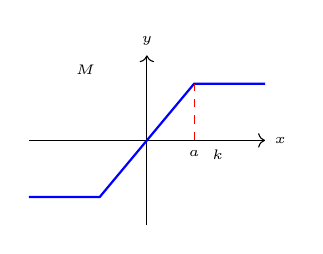
\begin{tikzpicture}[scale=0.6]
\draw[->] (-2.5,0) -- (2.5,0) node[right] {\tiny $x$};
\draw[->] (0,-1.8) -- (0,1.8) node[above] {\tiny $y$};
\draw[blue, thick] (-2.5,-1.2) -- (-1,-1.2) -- (1,1.2) -- (2.5,1.2);
\node at (1.5,-0.3) {\tiny $k$};
\node at (-1.3,1.5) {\tiny $M$};
\draw[dashed, red] (1,0) -- (1,1.2);
\node[below] at (1,0) {\tiny $a$};
\end{tikzpicture}
\end{center}

\begin{align*}
N(A) = \begin{cases}
k & A \leq a \\
\frac{2k}{\pi}\left[\arcsin\frac{a}{A} + \frac{a}{A}\sqrt{1-\left(\frac{a}{A}\right)^2}\right] & A > a
\end{cases}
\end{align*}

其中 $a = M/k$(饱和阈值)

\textbf{2. 死区特性}

\begin{align*}
N(A) = \begin{cases}
0 & A \leq \Delta \\
\frac{k}{\pi}\left[\pi - 2\arcsin\frac{\Delta}{A} - \frac{2\Delta}{A}\sqrt{1-\left(\frac{\Delta}{A}\right)^2}\right] & A > \Delta
\end{cases}
\end{align*}

\textbf{3. 继电特性}

\begin{align*}
N(A) = \frac{4M}{\pi A}
\end{align*}

$M$ 为继电器输出幅值
\end{minipage}

\subsubsection{稳定性分析}

\textbf{闭环系统结构:}

非线性环节 $N(A)$ 串联线性部分 $G(j\omega)$ 构成单位负反馈系统。

\textbf{稳定性判据(类似奈奎斯特判据):}

系统稳定的条件:
\begin{align*}
G(j\omega) \text{曲线不包围点} \left(-\frac{1}{N(A)}\right)
\end{align*}

\textbf{极限环判断:}

极限环存在的条件:
\begin{align*}
G(j\omega_0) = -\frac{1}{N(A_0)}
\end{align*}

此时系统产生频率为 $\omega_0$、幅值为 $A_0$ 的自激振荡。

\vspace{0.3cm}
\textbf{稳定性判断:}

\begin{itemize}
    \item 若 $-1/N(A)$ 曲线在 $G(j\omega)$ 外侧:稳定
    \item 若相交:存在极限环
    \item 极限环稳定性:由交点处曲线的相对位置决定
\end{itemize}

\vspace{0.3cm}
\textbf{例题:}系统含继电特性 $M=1$,线性部分 $G(s) = \frac{K}{s(s+1)}$,$K=2$,判断是否存在极限环。

\textit{解:}

\textbf{1. 继电特性的描述函数}
\begin{align*}
N(A) = \frac{4M}{\pi A} = \frac{4}{\pi A}
\end{align*}

\textbf{2. $-1/N(A)$ 曲线}
\begin{align*}
-\frac{1}{N(A)} = -\frac{\pi A}{4}
\end{align*}

这是实轴上的负半轴,$A$ 从 $0$ 到 $\infty$ 变化时,点从 $0$ 到 $-\infty$ 移动。

\textbf{3. $G(j\omega)$ 曲线}
\begin{align*}
G(j\omega) = \frac{2}{j\omega(1+j\omega)} = \frac{2(1-j\omega)}{\omega^2(1+\omega^2)}
\end{align*}

\textbf{4. 交点判断}

令 $\text{Im}[G(j\omega)] = 0$:$-2/[\omega^2(1+\omega^2)] = 0$ 无解

$G(j\omega)$ 曲线不与实轴负半轴相交 $\implies$ 不存在极限环。

\textbf{结论:}系统不会产生自激振荡。

\subsection{Lyapunov稳定性理论(非线性系统)}

Lyapunov第二方法(直接法)适用于非线性系统的稳定性分析,无需求解微分方程。

\subsubsection{Lyapunov稳定性定义}

考虑非线性系统:
\begin{align*}
\dot{\mathbf{x}} = \mathbf{f}(\mathbf{x}, t)
\end{align*}

假设 $\mathbf{x}_e$ 是平衡点($\mathbf{f}(\mathbf{x}_e, t) = 0$)。

\textbf{稳定性定义:}

\begin{itemize}
    \item \textbf{稳定}:对任意 $\epsilon > 0$,存在 $\delta > 0$,使得当 $\|\mathbf{x}(0) - \mathbf{x}_e\| < \delta$ 时,有 $\|\mathbf{x}(t) - \mathbf{x}_e\| < \epsilon$($t \geq 0$)
    \item \textbf{渐近稳定}:稳定且 $\lim_{t\to\infty} \mathbf{x}(t) = \mathbf{x}_e$
    \item \textbf{全局渐近稳定}:对任意初始条件都渐近稳定
\end{itemize}

\subsubsection{Lyapunov定理}

\textbf{定理(Lyapunov稳定性定理):}

如果存在标量函数 $V(\mathbf{x})$(Lyapunov函数)满足:

\begin{enumerate}
    \item $V(\mathbf{x})$ 连续可微
    \item $V(\mathbf{x}_e) = 0$ 且在 $\mathbf{x} \neq \mathbf{x}_e$ 时 $V(\mathbf{x}) > 0$(正定)
    \item $\dot{V}(\mathbf{x}) = \frac{\partial V}{\partial \mathbf{x}} \cdot \mathbf{f}(\mathbf{x}, t) \leq 0$(半负定)
\end{enumerate}

则平衡点 $\mathbf{x}_e$ 是\textbf{稳定}的。

如果进一步满足:
\begin{enumerate}
    \setcounter{enumi}{3}
    \item $\dot{V}(\mathbf{x}) < 0$($\mathbf{x} \neq \mathbf{x}_e$,负定)
\end{enumerate}

则平衡点 $\mathbf{x}_e$ 是\textbf{渐近稳定}的。

\vspace{0.3cm}
\textbf{Lyapunov函数的构造:}

常用形式(二次型):
\begin{align*}
V(\mathbf{x}) = \mathbf{x}^T \mathbf{P} \mathbf{x}
\end{align*}

其中 $\mathbf{P}$ 是正定对称矩阵。

\vspace{0.3cm}
\textbf{例题:}分析系统 $\dot{x}_1 = x_2$,$\dot{x}_2 = -x_1 - x_2$ 的稳定性。

\textit{解:}

\textbf{1. 确定平衡点}

令 $\dot{x}_1 = \dot{x}_2 = 0$:$x_1 = x_2 = 0$

\textbf{2. 构造Lyapunov函数}

选择:$V(x_1, x_2) = x_1^2 + x_2^2$

\textbf{3. 验证正定性}

$V(0, 0) = 0$ 且 $V(x_1, x_2) > 0$($x_1, x_2$ 不全为零)$\implies$ 正定

\textbf{4. 计算 $\dot{V}$}
\begin{align*}
\dot{V} &= \frac{\partial V}{\partial x_1}\dot{x}_1 + \frac{\partial V}{\partial x_2}\dot{x}_2 \\
&= 2x_1 \cdot x_2 + 2x_2 \cdot (-x_1 - x_2) \\
&= 2x_1 x_2 - 2x_1 x_2 - 2x_2^2 \\
&= -2x_2^2 \leq 0
\end{align*}

$\dot{V} < 0$(除原点外)$\implies$ 负定

\textbf{结论:}原点是\textbf{渐近稳定}的平衡点。

\subsection{总结}

\begin{center}
\begin{tabular}{|l|p{4cm}|p{4cm}|p{3cm}|}
\hline
\textbf{方法} & \textbf{适用范围} & \textbf{优点} & \textbf{缺点} \\
\hline
相平面法 & 二阶系统 & 直观、图形化 & 仅限二阶 \\
\hline
描述函数法 & 含单一非线性环节 & 频域分析、预测极限环 & 近似方法 \\
\hline
Lyapunov法 & 任意阶非线性系统 & 严格、不需求解方程 & 构造函数困难 \\
\hline
\end{tabular}
\end{center}

\section{离散系统}

\subsection{离散系统概述}

\subsubsection{离散系统的定义}

\textbf{离散系统}(数字控制系统)是指信号在时间上离散,通常涉及采样、数字处理和保持等环节。

\begin{minipage}[t]{0.52\textwidth}
\textbf{连续系统 vs 离散系统:}

\textbf{连续系统:}
\begin{itemize}
    \item 信号连续变化
    \item 微分方程描述
    \item 拉普拉斯变换分析
\end{itemize}

\textbf{离散系统:}
\begin{itemize}
    \item 信号在采样时刻定义
    \item 差分方程描述
    \item Z变换分析
\end{itemize}

\vspace{0.3cm}
\textbf{离散系统的组成:}

\begin{enumerate}
    \item \textbf{采样器}:将连续信号转换为离散序列
    \item \textbf{数字控制器}:对离散信号进行数字处理
    \item \textbf{保持器}:将离散信号还原为连续信号
    \item \textbf{被控对象}:连续系统
\end{enumerate}

\vspace{0.3cm}
\textbf{采样定理(Nyquist-Shannon定理):}

为无失真恢复连续信号,采样频率必须:
\begin{align*}
f_s \geq 2f_{\max}
\end{align*}

或采样周期:
\begin{align*}
T \leq \frac{\pi}{\omega_{\max}}
\end{align*}

其中 $f_{\max}$ 是信号的最高频率分量。

\textbf{工程实践:}
\begin{itemize}
    \item 一般取 $f_s = (6 \sim 10) f_{\max}$
    \item 或采样周期 $T = (0.1 \sim 0.5) T_s$($T_s$ 为系统时间常数)
\end{itemize}
\end{minipage}\hfill
\begin{minipage}[t]{0.45\textwidth}
\vspace{0pt}
\textbf{离散控制系统结构:}

离散控制系统包含以下环节:
\begin{itemize}
    \item 采样器(周期 $T$)
    \item 数字控制器
    \item 保持器(通常为零阶保持器)
    \item 被控对象(连续系统)
\end{itemize}

采样器将连续信号在离散时刻采样,数字控制器对离散信号进行处理,保持器将离散信号还原为阶梯波形式的连续信号,最后作用于被控对象。

\vspace{0.3cm}
\textbf{采样过程:}

采样过程将连续信号 $r(t)$ 在时刻 $t = kT$($k=0,1,2,\ldots$)进行采样,得到离散序列 $r(kT)$。
\end{minipage}

\subsection{Z变换}

Z变换是分析离散系统的数学工具,类似于连续系统中的拉普拉斯变换。

\subsubsection{Z变换的定义}

对于离散序列 $\{f(kT)\}$($k = 0, 1, 2, \ldots$),其Z变换定义为:
\begin{align*}
F(z) = \mathcal{Z}\{f(kT)\} = \sum_{k=0}^{\infty} f(kT) z^{-k}
\end{align*}

其中 $z$ 是复变量。

\subsubsection{Z变换与拉氏变换的关系}

对于采样信号 $f^*(t) = \sum_{k=0}^{\infty} f(kT)\delta(t-kT)$,其拉氏变换为:
\begin{align*}
F^*(s) = \sum_{k=0}^{\infty} f(kT) e^{-skT}
\end{align*}

令 $z = e^{sT}$,则:
\begin{align*}
F(z) = F^*(s)\Big|_{z=e^{sT}}
\end{align*}

\textbf{$s$ 平面与 $z$ 平面的映射:}

\begin{center}
\begin{tikzpicture}[scale=0.7]
% s平面
\begin{scope}[shift={(0,0)}]
\draw[->] (-2,0) -- (2,0) node[right] {$\text{Re}(s)$};
\draw[->] (0,-2) -- (0,2) node[above] {$\text{Im}(s)$};
\draw[blue, thick] (-2,-2) -- (-2,2);
\draw[red, thick] (0,-2) -- (0,2);
\node[blue, left] at (-2,1.5) {不稳定};
\node[red, right] at (0,1.5) {稳定};
\node[below] at (0,-2.5) {$s$ 平面};
\end{scope}

% 箭头
\draw[->, thick] (2.5,0) -- (3.5,0) node[midway, above] {\small $z=e^{sT}$};

% z平面
\begin{scope}[shift={(6,0)}]
\draw[->] (-2,0) -- (2,0) node[right] {$\text{Re}(z)$};
\draw[->] (0,-2) -- (0,2) node[above] {$\text{Im}(z)$};
\draw[thick] (0,0) circle (1);
\fill[blue, opacity=0.2] (0,0) circle (1);
\node[red] at (1.5,0) {不稳定};
\node[blue] at (0.5,0.5) {稳定};
\node[below] at (0,-2.5) {$z$ 平面};
\end{scope}
\end{tikzpicture}
\end{center}

\textbf{关键对应关系:}
\begin{itemize}
    \item $s$ 平面左半平面 $\leftrightarrow$ $z$ 平面单位圆内
    \item $s$ 平面虚轴 $\leftrightarrow$ $z$ 平面单位圆上
    \item $s$ 平面右半平面 $\leftrightarrow$ $z$ 平面单位圆外
\end{itemize}

\subsubsection{常用序列的Z变换}

\begin{center}
\begin{tabular}{|c|c|c|}
\hline
\textbf{序列} $f(kT)$ & \textbf{Z变换} $F(z)$ & \textbf{收敛域} \\
\hline
$\delta(kT)$(单位脉冲) & $1$ & 全平面 \\
\hline
$1(kT)$(单位阶跃) & $\frac{z}{z-1}$ & $|z| > 1$ \\
\hline
$kT$ & $\frac{Tz}{(z-1)^2}$ & $|z| > 1$ \\
\hline
$e^{-akT}$ & $\frac{z}{z-e^{-aT}}$ & $|z| > e^{-aT}$ \\
\hline
$\sin(\omega kT)$ & $\frac{z\sin(\omega T)}{z^2 - 2z\cos(\omega T) + 1}$ & $|z| > 1$ \\
\hline
$\cos(\omega kT)$ & $\frac{z[z-\cos(\omega T)]}{z^2 - 2z\cos(\omega T) + 1}$ & $|z| > 1$ \\
\hline
$a^k$ & $\frac{z}{z-a}$ & $|z| > |a|$ \\
\hline
$ka^k$ & $\frac{az}{(z-a)^2}$ & $|z| > |a|$ \\
\hline
\end{tabular}
\end{center}

\subsubsection{Z变换的性质}

\begin{center}
\begin{tabular}{|l|c|c|}
\hline
\textbf{性质} & \textbf{时域} & \textbf{Z域} \\
\hline
线性 & $a f_1(kT) + b f_2(kT)$ & $a F_1(z) + b F_2(z)$ \\
\hline
右移 & $f(kT - nT)$ & $z^{-n} F(z)$ \\
\hline
左移 & $f(kT + nT)$ & $z^n [F(z) - \sum_{k=0}^{n-1} f(kT) z^{-k}]$ \\
\hline
初值定理 & $f(0)$ & $\lim_{z\to\infty} F(z)$ \\
\hline
终值定理 & $\lim_{k\to\infty} f(kT)$ & $\lim_{z\to 1} (z-1)F(z)$ \\
\hline
卷积 & $\sum_{i=0}^k f_1(iT) f_2(kT-iT)$ & $F_1(z) \cdot F_2(z)$ \\
\hline
\end{tabular}
\end{center}

\subsection{脉冲传递函数}

\subsubsection{定义}

脉冲传递函数是离散系统的输出Z变换与输入Z变换之比(零初始条件):
\begin{align*}
G(z) = \frac{Y(z)}{X(z)}
\end{align*}

\subsubsection{零阶保持器(ZOH)}

零阶保持器在采样周期内保持采样值不变。

\begin{minipage}[t]{0.52\textwidth}
\textbf{零阶保持器的传递函数:}
\begin{align*}
G_h(s) = \frac{1 - e^{-Ts}}{s}
\end{align*}

\textbf{含零阶保持器的系统:}

采样器 + ZOH + 连续对象 $G(s)$

等效脉冲传递函数:
\begin{align*}
G(z) = \mathcal{Z}\left\{\frac{1-e^{-Ts}}{s} G(s)\right\} = (1-z^{-1})\mathcal{Z}\left\{\frac{G(s)}{s}\right\}
\end{align*}

\vspace{0.3cm}
\textbf{常用公式:}

对于 $G(s) = \frac{1}{s+a}$:
\begin{align*}
G(z) = (1-z^{-1})\mathcal{Z}\left\{\frac{1}{s(s+a)}\right\} = \frac{1-e^{-aT}}{z-e^{-aT}}
\end{align*}

对于 $G(s) = \frac{1}{s(s+a)}$:
\begin{align*}
G(z) = (1-z^{-1})\mathcal{Z}\left\{\frac{1}{s^2(s+a)}\right\} = \frac{T - \frac{1-e^{-aT}}{a}}{(z-1)(z-e^{-aT})}
\end{align*}
\end{minipage}\hfill
\begin{minipage}[t]{0.45\textwidth}
\vspace{0pt}
\textbf{零阶保持器输出示意:}

零阶保持器(Zero-Order Hold, ZOH)在每个采样周期内保持采样值不变,将离散信号转换为阶梯波形式的连续信号。

输出特点:
\begin{itemize}
    \item 在每个采样周期 $[kT, (k+1)T)$ 内,输出保持为 $y(kT)$
    \item 在采样时刻发生跳变
    \item 形成阶梯波形
\end{itemize}

\vspace{0.5cm}
\textbf{例题:}求含ZOH和对象 $G(s) = \frac{1}{s+2}$ 的脉冲传递函数,$T = 0.1$ s。

\textit{解:}

\textbf{方法1:查表法}
\begin{align*}
G(z) &= (1-z^{-1})\mathcal{Z}\left\{\frac{1}{s(s+2)}\right\} \\
&= \frac{1-e^{-2T}}{z-e^{-2T}} \\
&= \frac{1-e^{-0.2}}{z-e^{-0.2}} \\
&= \frac{0.1813}{z-0.8187}
\end{align*}

\textbf{方法2:部分分式法}
\begin{align*}
\frac{G(s)}{s} &= \frac{1}{s(s+2)} = \frac{0.5}{s} - \frac{0.5}{s+2} \\
\mathcal{Z}\left\{\frac{1}{s(s+2)}\right\} &= 0.5\frac{z}{z-1} - 0.5\frac{z}{z-e^{-2T}} \\
G(z) &= (1-z^{-1}) \times \text{上式} \\
&= \frac{0.1813}{z-0.8187}
\end{align*}
\end{minipage}

\subsection{离散系统的稳定性}

\subsubsection{稳定性判据}

离散系统稳定的充要条件:闭环脉冲传递函数 $\Phi(z)$ 的所有极点都在 $z$ 平面单位圆内,即:
\begin{align*}
|z_i| < 1, \quad i = 1, 2, \ldots, n
\end{align*}

\subsubsection{劳斯判据的应用(双线性变换)}

通过双线性变换 $z = \frac{1+w}{1-w}$,将 $z$ 平面单位圆内映射到 $w$ 平面左半平面,然后应用劳斯判据。

\textbf{步骤:}

1. 求闭环特征方程 $D(z) = 0$

2. 进行双线性变换:$z = \frac{1+w}{1-w}$,得 $D(w) = 0$

3. 对 $D(w) = 0$ 应用劳斯判据

\vspace{0.3cm}
\textbf{例题:}判断系统 $\Phi(z) = \frac{K}{z^2 - 1.5z + 0.5}$ 的稳定性,$K = 1$。

\textit{解:}

\textbf{1. 特征方程}
\begin{align*}
D(z) = z^2 - 1.5z + 0.5 + K = z^2 - 1.5z + 1.5 = 0
\end{align*}

\textbf{2. 双线性变换}

令 $z = \frac{1+w}{1-w}$:
\begin{align*}
\left(\frac{1+w}{1-w}\right)^2 - 1.5\frac{1+w}{1-w} + 1.5 &= 0 \\
(1+w)^2 - 1.5(1+w)(1-w) + 1.5(1-w)^2 &= 0 \\
1 + 2w + w^2 - 1.5(1-w^2) + 1.5(1-2w+w^2) &= 0 \\
1 + 2w + w^2 - 1.5 + 1.5w^2 + 1.5 - 3w + 1.5w^2 &= 0 \\
4w^2 - w + 1 &= 0
\end{align*}

\textbf{3. 劳斯表}
\begin{center}
\begin{tabular}{c|cc}
$w^2$ & 4 & 1 \\
$w^1$ & -1 & 0 \\
$w^0$ & 1 &  \\
\end{tabular}
\end{center}

第一列有符号变化(+,-,+)$\implies$ \textbf{不稳定}

\textbf{验证:}直接求根:$z = \frac{1.5 \pm \sqrt{2.25-6}}{2} = 0.75 \pm 0.968j$,$|z| = 1.22 > 1$

\subsubsection{Jury稳定性判据}

Jury判据直接在 $z$ 域判断稳定性,无需变换。

设特征方程:
\begin{align*}
D(z) = a_0 z^n + a_1 z^{n-1} + \cdots + a_{n-1} z + a_n = 0
\end{align*}

\textbf{稳定的必要条件:}
\begin{align*}
D(1) > 0, \quad (-1)^n D(-1) > 0
\end{align*}

\textbf{充要条件:}构造Jury表,所有行的首元素满足特定符号条件。

(详细方法略,工程中常用数值计算求根判断)

\subsection{离散系统的动态性能}

\subsubsection{稳态误差}

\textbf{终值定理:}
\begin{align*}
e_{ss} = \lim_{k\to\infty} e(kT) = \lim_{z\to 1} (z-1)E(z)
\end{align*}

\textbf{单位阶跃输入:}$R(z) = \frac{z}{z-1}$
\begin{align*}
e_{ss} = \lim_{z\to 1} (z-1) \frac{R(z)}{1+G(z)} = \frac{1}{1 + \lim_{z\to 1} G(z)}
\end{align*}

\textbf{单位斜坡输入:}$R(z) = \frac{Tz}{(z-1)^2}$
\begin{align*}
e_{ss} = \lim_{z\to 1} (z-1) \frac{Tz}{(z-1)^2[1+G(z)]} = \frac{T}{\lim_{z\to 1} (z-1)G(z)/T}
\end{align*}

\subsubsection{瞬态性能指标}

离散系统的时域响应可以通过Z反变换求得:
\begin{align*}
y(kT) = \mathcal{Z}^{-1}\{Y(z)\}
\end{align*}

\textbf{常用方法:}
\begin{itemize}
    \item \textbf{长除法}:直接展开为序列
    \item \textbf{部分分式法}:分解后查表反变换
    \item \textbf{留数法}:复变函数理论
\end{itemize}

\textbf{性能指标:}
\begin{itemize}
    \item 上升时间 $t_r$
    \item 超调量 $\sigma\%$
    \item 调节时间 $t_s$
    \item 振荡次数
\end{itemize}

\subsection{数字PID控制}

\subsubsection{连续PID的离散化}

连续PID控制器:
\begin{align*}
u(t) = K_p e(t) + K_i \int_0^t e(\tau) d\tau + K_d \frac{de(t)}{dt}
\end{align*}

\textbf{位置式数字PID:}
\begin{align*}
u(k) = K_p e(k) + K_i T \sum_{j=0}^k e(j) + K_d \frac{e(k) - e(k-1)}{T}
\end{align*}

\textbf{速度式数字PID:}
\begin{align*}
\Delta u(k) = u(k) - u(k-1) &= K_p [e(k) - e(k-1)] \\
&\quad + K_i T e(k) \\
&\quad + K_d \frac{e(k) - 2e(k-1) + e(k-2)}{T}
\end{align*}

\subsubsection{数字PID的改进}

\textbf{1. 积分分离}:误差大时不积分,避免积分饱和
\begin{align*}
u(k) = K_p e(k) + K_i T \sum_{j=k_0}^k e(j) + K_d \frac{e(k) - e(k-1)}{T}
\end{align*}

\textbf{2. 微分先行}:仅对输出微分,避免对设定值突变响应过大
\begin{align*}
u(k) = K_p e(k) + K_i T \sum_{j=0}^k e(j) - K_d \frac{y(k) - y(k-1)}{T}
\end{align*}

\textbf{3. 不完全微分}:加入滤波环节,减小噪声影响
\begin{align*}
u_d(k) = \alpha u_d(k-1) + K_d (1-\alpha) \frac{e(k) - e(k-1)}{T}
\end{align*}

其中 $\alpha = \frac{T}{T + \tau_d}$,$\tau_d$ 为滤波时间常数。

\subsection{离散系统设计}

\subsubsection{最少拍控制}

\textbf{设计目标:}在最少的采样周期内使系统输出达到并保持在期望值。

\textbf{设计步骤:}

1. 确定期望闭环传递函数 $\Phi^*(z)$

2. 计算控制器传递函数:
\begin{align*}
D(z) = \frac{\Phi^*(z)}{G(z)[1-\Phi^*(z)]}
\end{align*}

3. 验证物理可实现性和稳定性

\textbf{常用期望响应:}
\begin{itemize}
    \item 单拍系统:$\Phi^*(z) = z^{-1}$
    \item 有纹波最少拍:$\Phi^*(z) = \frac{(1-a)z^{-1}}{1-az^{-1}}$
    \item 无纹波最少拍(I型系统):$\Phi^*(z) = z^{-1}(2-z^{-1})$
\end{itemize}

\subsubsection{数字控制器的实现}

\textbf{直接编程法:}

控制器传递函数 $D(z) = \frac{U(z)}{E(z)}$ 转换为差分方程,直接编程实现。

\textbf{串行校正:}

类似连续系统的超前/滞后校正,设计数字校正器:
\begin{align*}
D(z) = K \frac{z - a}{z - b}
\end{align*}

\textbf{并行校正:}

采用状态反馈等现代控制方法。

\subsection{总结}

\begin{center}
\begin{tabular}{|l|c|c|}
\hline
\textbf{特性} & \textbf{连续系统} & \textbf{离散系统} \\
\hline
数学描述 & 微分方程 & 差分方程 \\
\hline
变换工具 & 拉普拉斯变换 & Z变换 \\
\hline
频域函数 & 传递函数 $G(s)$ & 脉冲传递函数 $G(z)$ \\
\hline
稳定域 & $s$ 平面左半平面 & $z$ 平面单位圆内 \\
\hline
稳定判据 & 劳斯、奈奎斯特 & 双线性变换+劳斯、Jury \\
\hline
控制器 & 模拟PID & 数字PID、最少拍 \\
\hline
\end{tabular}
\end{center}

\textbf{离散系统设计要点:}
\begin{enumerate}
    \item 选择合适的采样周期(满足采样定理,通常 $T = 0.1 \sim 0.5$ 时间常数)
    \item 考虑零阶保持器的影响
    \item 数字控制器设计(数字PID、最少拍等)
    \item 验证闭环稳定性(极点在单位圆内)
    \item 评估动态性能(超调、调节时间等)
\end{enumerate}


\part{现代控制理论}

\section{状态空间表达式及其建立}

\subsection{状态空间的基本概念}
\begin{itemize}
    \item \textbf{状态}:系统在某一时刻的状态是指确定系统该时刻以后行为所必需的最少信息
    \item \textbf{状态变量}:描述系统状态的一组变量
    \item \textbf{状态向量}:由状态变量组成的向量
    \item \textbf{状态空间}:以状态变量为坐标的n维空间
\end{itemize}

\subsection{状态空间表达式}
线性定常系统的状态空间表达式:
\begin{align}
\dot{x}(t) &= Ax(t) + Bu(t) \\
\dot{y}(t) &= Cx(t) + Du(t)
\end{align}

其中:
\begin{itemize}
    \item $x(t) \in \mathbb{R}^n$:状态向量
    \item $u(t) \in \mathbb{R}^p$:输入向量
    \item $y(t) \in \mathbb{R}^q$:输出向量
    \item $A \in \mathbb{R}^{n \times n}$:系统矩阵
    \item $B \in \mathbb{R}^{n \times p}$:输入矩阵
    \item $C \in \mathbb{R}^{q \times n}$:输出矩阵
    \item $D \in \mathbb{R}^{q \times p}$:前馈矩阵
\end{itemize}

\subsection{状态空间表达式的建立方法}
\begin{enumerate}
    \item 根据物理规律建立微分方程组
    \item 选择状态变量(通常选择能量存储元件的变量)
    \item 将高阶微分方程化为一阶微分方程组
    \item 写出输出方程
\end{enumerate}

\section{状态空间表达式求传递函数}

\subsection{传递函数矩阵}
从状态空间表达式求传递函数矩阵:
\[G(s) = C(sI - A)^{-1}B + D\]

\subsection{单输入单输出系统}
对于单输入单输出系统:
\[G(s) = C(sI - A)^{-1}B + D\]

其中 $(sI - A)^{-1}$ 称为系统的解析矩阵。

\section{线性变换}

\subsection{线性变换的定义}
设 $x$ 和 $z$ 是两组状态变量,如果存在非奇异矩阵 $P$,使得:
\[x = Pz\]
则称此变换为线性变换或坐标变换。

\subsection{变换后的状态方程}
原系统:
\begin{align}
\dot{x} &= Ax + Bu \\
y &= Cx + Du
\end{align}

变换后的系统:
\begin{align}
\dot{z} &= \bar{A}z + \bar{B}u \\
y &= \bar{C}z + Du
\end{align}

其中:
\begin{align}
\bar{A} &= P^{-1}AP \\
\bar{B} &= P^{-1}B \\
\bar{C} &= CP
\end{align}


\section{线性控制系统状态空间表达式的求解}

\subsection{齐次状态方程的解}
齐次状态方程 $\dot{x} = Ax$ 的解为:
\[x(t) = e^{At}x(0)\]

其中 $e^{At}$ 称为状态转移矩阵,记为 $\Phi(t)$。

\subsection{状态转移矩阵的性质}
\begin{enumerate}
    \item $\Phi(0) = I$
    \item $\Phi(t_1 + t_2) = \Phi(t_1)\Phi(t_2)$
    \item $\Phi^{-1}(t) = \Phi(-t)$
    \item $\frac{d\Phi(t)}{dt} = A\Phi(t) = \Phi(t)A$
\end{enumerate}

\subsection{状态转移矩阵的计算方法}
\begin{enumerate}
    \item 级数展开法:$e^{At} = I + At + \frac{A^2t^2}{2!} + \cdots$
    \item 拉普拉斯变换法:$e^{At} = \mathcal{L}^{-1}[(sI-A)^{-1}]$
    \item 对角化方法:当 $A$ 可对角化时
    \item 约当标准形方法:当 $A$ 不可对角化时
\end{enumerate}

\subsection{非齐次状态方程的解}
非齐次状态方程的完全解:
\[x(t) = e^{At}x(0) + \int_0^t e^{A(t-\tau)}Bu(\tau)d\tau\]
\section{线性控制系统的能控性和能观测性}

\subsection{能控性定义}
系统 $(A, B)$ 在时刻 $t_0$ 是状态能控的,如果存在有限时间 $t_1 > t_0$ 和控制输入 $u(t)$,使得系统能从任意初态 $x(t_0)$ 转移到任意终态 $x(t_1)$。

\subsection{能控性判据}
系统 $(A, B)$ 完全能控的充要条件是能控性矩阵:
\[W_c = [B \quad AB \quad A^2B \quad \cdots \quad A^{n-1}B]\]
满足 $\text{rank}(W_c) = n$。

\subsection{能观测性定义}
系统 $(A, C)$ 在时刻 $t_0$ 是状态能观测的,如果能够根据有限时间区间 $[t_0, t_1]$ 内的输出 $y(t)$ 和输入 $u(t)$ 唯一地确定初始状态 $x(t_0)$。

\subsection{能观测性判据}
系统 $(A, C)$ 完全能观测的充要条件是能观测性矩阵:
\[W_o = \begin{bmatrix}
C \\ CA \\ CA^2 \\ \vdots \\ CA^{n-1}
\end{bmatrix}\]
满足 $\text{rank}(W_o) = n$。


\section{能控、能观标准型及其实现}

\subsection{能控标准型}
对于单输入系统,能控标准型为:
\[\bar{A} = \begin{bmatrix}
0 & 1 & 0 & \cdots & 0 \\
0 & 0 & 1 & \cdots & 0 \\
\vdots & \vdots & \vdots & \ddots & \vdots \\
0 & 0 & 0 & \cdots & 1 \\
-a_0 & -a_1 & -a_2 & \cdots & -a_{n-1}
\end{bmatrix}, \quad \bar{B} = \begin{bmatrix} 0 \\ 0 \\ \vdots \\ 0 \\ 1 \end{bmatrix}\]

\subsection{能观测标准型}
对于单输出系统,能观测标准型为:
\[\bar{A} = \begin{bmatrix}
0 & 0 & \cdots & 0 & -a_0 \\
1 & 0 & \cdots & 0 & -a_1 \\
0 & 1 & \cdots & 0 & -a_2 \\
\vdots & \vdots & \ddots & \vdots & \vdots \\
0 & 0 & \cdots & 1 & -a_{n-1}
\end{bmatrix}, \quad \bar{C} = \begin{bmatrix} 0 & 0 & \cdots & 0 & 1 \end{bmatrix}\]

\section{系统的结构分解——能控、能观性分解}

\subsection{系统的结构分解}
一般线性系统可分解为四个子系统:
\begin{itemize}
    \item 能控且能观测部分
    \item 能控但不能观测部分
    \item 不能控但能观测部分
    \item 不能控且不能观测部分
\end{itemize}

\subsection{卡尔曼分解}
通过适当的线性变换,可将系统分解为:
\[\begin{bmatrix} \dot{x}_1 \\ \dot{x}_2 \\ \dot{x}_3 \\ \dot{x}_4 \end{bmatrix} = 
\begin{bmatrix}
A_{11} & 0 & A_{13} & 0 \\
A_{21} & A_{22} & A_{23} & A_{24} \\
0 & 0 & A_{33} & 0 \\
0 & 0 & A_{43} & A_{44}
\end{bmatrix}
\begin{bmatrix} x_1 \\ x_2 \\ x_3 \\ x_4 \end{bmatrix} +
\begin{bmatrix} B_1 \\ B_2 \\ 0 \\ 0 \end{bmatrix} u\]

\[y = \begin{bmatrix} C_1 & C_2 & 0 & 0 \end{bmatrix} \begin{bmatrix} x_1 \\ x_2 \\ x_3 \\ x_4 \end{bmatrix}\]

\section{约当型实现}

\subsection{约当标准型}
当系统矩阵 $A$ 的特征值不同时,可化为对角形:
\[J = P^{-1}AP = \text{diag}(\lambda_1, \lambda_2, \ldots, \lambda_n)\]

当有重根时,化为约当标准型:
\[J = P^{-1}AP = \text{diag}(J_1, J_2, \ldots, J_k)\]

其中 $J_i$ 为约当块:
\[J_i = \begin{bmatrix}
\lambda_i & 1 & 0 & \cdots & 0 \\
0 & \lambda_i & 1 & \cdots & 0 \\
\vdots & \vdots & \vdots & \ddots & \vdots \\
0 & 0 & 0 & \cdots & \lambda_i
\end{bmatrix}\]

\section{稳定性与李雅普诺夫方法}

\subsection{李雅普诺夫稳定性定义}
考虑自治系统 $\dot{x} = f(x)$,设 $x_e$ 为平衡点:
\begin{itemize}
    \item \textbf{稳定}:对任意 $\varepsilon > 0$,存在 $\delta > 0$,当 $\|x(0) - x_e\| < \delta$ 时,有 $\|x(t) - x_e\| < \varepsilon$,$\forall t \geq 0$
    \item \textbf{渐近稳定}:稳定且 $\lim_{t \to \infty} x(t) = x_e$
    \item \textbf{大范围渐近稳定}:渐近稳定且吸引域为整个状态空间
\end{itemize}

\subsection{李雅普诺夫第一方法(线性化方法)}
对于线性系统 $\dot{x} = Ax$,系统渐近稳定的充要条件是矩阵 $A$ 的所有特征值都具有负实部。

\subsection{李雅普诺夫第二方法(直接方法)}
\textbf{李雅普诺夫定理}:如果存在标量函数 $V(x)$ 满足:
\begin{enumerate}
    \item $V(x)$ 连续且有连续的一阶偏导数
    \item $V(x_e) = 0$,当 $x \neq x_e$ 时 $V(x) > 0$(正定)
    \item $\dot{V}(x) = \frac{\partial V}{\partial x} f(x) \leq 0$(半负定)
\end{enumerate}
则平衡点 $x_e$ 稳定。

若进一步有 $\dot{V}(x) < 0$(负定),则平衡点渐近稳定。

\subsection{线性系统的李雅普诺夫方程}
对于线性系统 $\dot{x} = Ax$,选择二次型李雅普诺夫函数:
\[V(x) = x^T P x\]

其中 $P$ 为正定矩阵。稳定的充要条件是李雅普诺夫方程:
\[A^T P + PA = -Q\]
对于给定的正定矩阵 $Q$,存在唯一的正定解 $P$。

\section{极点配置——状态反馈}

\subsection{状态反馈}
状态反馈控制律:
\[u = -Kx + v\]

其中 $K$ 为反馈增益矩阵,$v$ 为参考输入。

闭环系统:
\[\dot{x} = (A - BK)x + Bv\]

\subsection{极点配置定理}
对于单输入系统,若 $(A, B)$ 完全能控,则对于任意给定的 $n$ 个复数 $\lambda_1, \lambda_2, \ldots, \lambda_n$(复数成对共轭出现),存在反馈增益矩阵 $K$,使得闭环系统矩阵 $A - BK$ 的特征值恰好为 $\lambda_1, \lambda_2, \ldots, \lambda_n$。

\subsection{极点配置的方法}
\begin{enumerate}
    \item \textbf{直接方法}:解特征方程 $\det(sI - A + BK) = 0$
    \item \textbf{变换方法}:将系统化为能控标准型后配置极点
    \item \textbf{阿克曼公式}:$K = [0 \quad 0 \quad \cdots \quad 0 \quad 1] W_c^{-1} \alpha_c(A)$
\end{enumerate}

其中 $\alpha_c(s)$ 为期望的特征多项式,$W_c$ 为能控性矩阵。

\section{状态观测器}

\subsection{状态观测器的概念}
当系统的状态不能直接测量时,需要根据系统的输入输出信息来估计状态变量,这种估计装置称为状态观测器。

\subsection{全维状态观测器}
全维状态观测器的方程:
\[\dot{\hat{x}} = A\hat{x} + Bu + L(y - C\hat{x})\]

其中 $\hat{x}$ 为状态估计值,$L$ 为观测器增益矩阵。

\subsection{观测器的设计}
观测误差:$e = x - \hat{x}$

观测误差动态方程:
\[\dot{e} = (A - LC)e\]

观测器设计就是选择 $L$,使得 $A - LC$ 的特征值位于左半平面。

\textbf{观测器设计定理}:若 $(A, C)$ 完全能观测,则可任意配置观测器的极点。

\subsection{分离定理}
状态反馈与状态观测器可以分别独立设计,即:
\begin{itemize}
    \item 先设计状态反馈增益 $K$,配置闭环系统的极点
    \item 再设计观测器增益 $L$,配置观测器的极点
\end{itemize}

基于观测器的状态反馈系统的特征多项式等于控制器特征多项式与观测器特征多项式的乘积。


\end{document}
